\documentclass[11pt]{article}
\usepackage[utf8]{inputenc}
\usepackage[a4paper, total={6in, 10in}]{geometry}
\usepackage{graphicx} % Required for inserting images
\usepackage[italian]{babel}
\usepackage{float}
\usepackage[table]{xcolor}
\usepackage{tabularx}
\usepackage{hyperref}
\usepackage{listings}
\usepackage{color}
\usepackage{tcolorbox}

\lstdefinestyle{sqlStyle}{
    language=SQL,
    basicstyle=\ttfamily\footnotesize, 
    keywordstyle=\color{blue},
    stringstyle=\color{red},
    commentstyle=\color{gray},
    morecomment=[l][\color{magenta}]{\#},
    morekeywords={INSERT, INTO, VALUES},
    breaklines=true,
    showstringspaces=false,
    numbers=left,
    frame=none,
    numberstyle=\small,
    numbersep=-18pt,
    xleftmargin=-13pt,
}


\title{Dealership ``Elite" Data Base}
\author{Elvis Perlika}
\date{\today}

\begin{document}

\maketitle

\vspace{0.8in}

\begin{center}
    \centering
    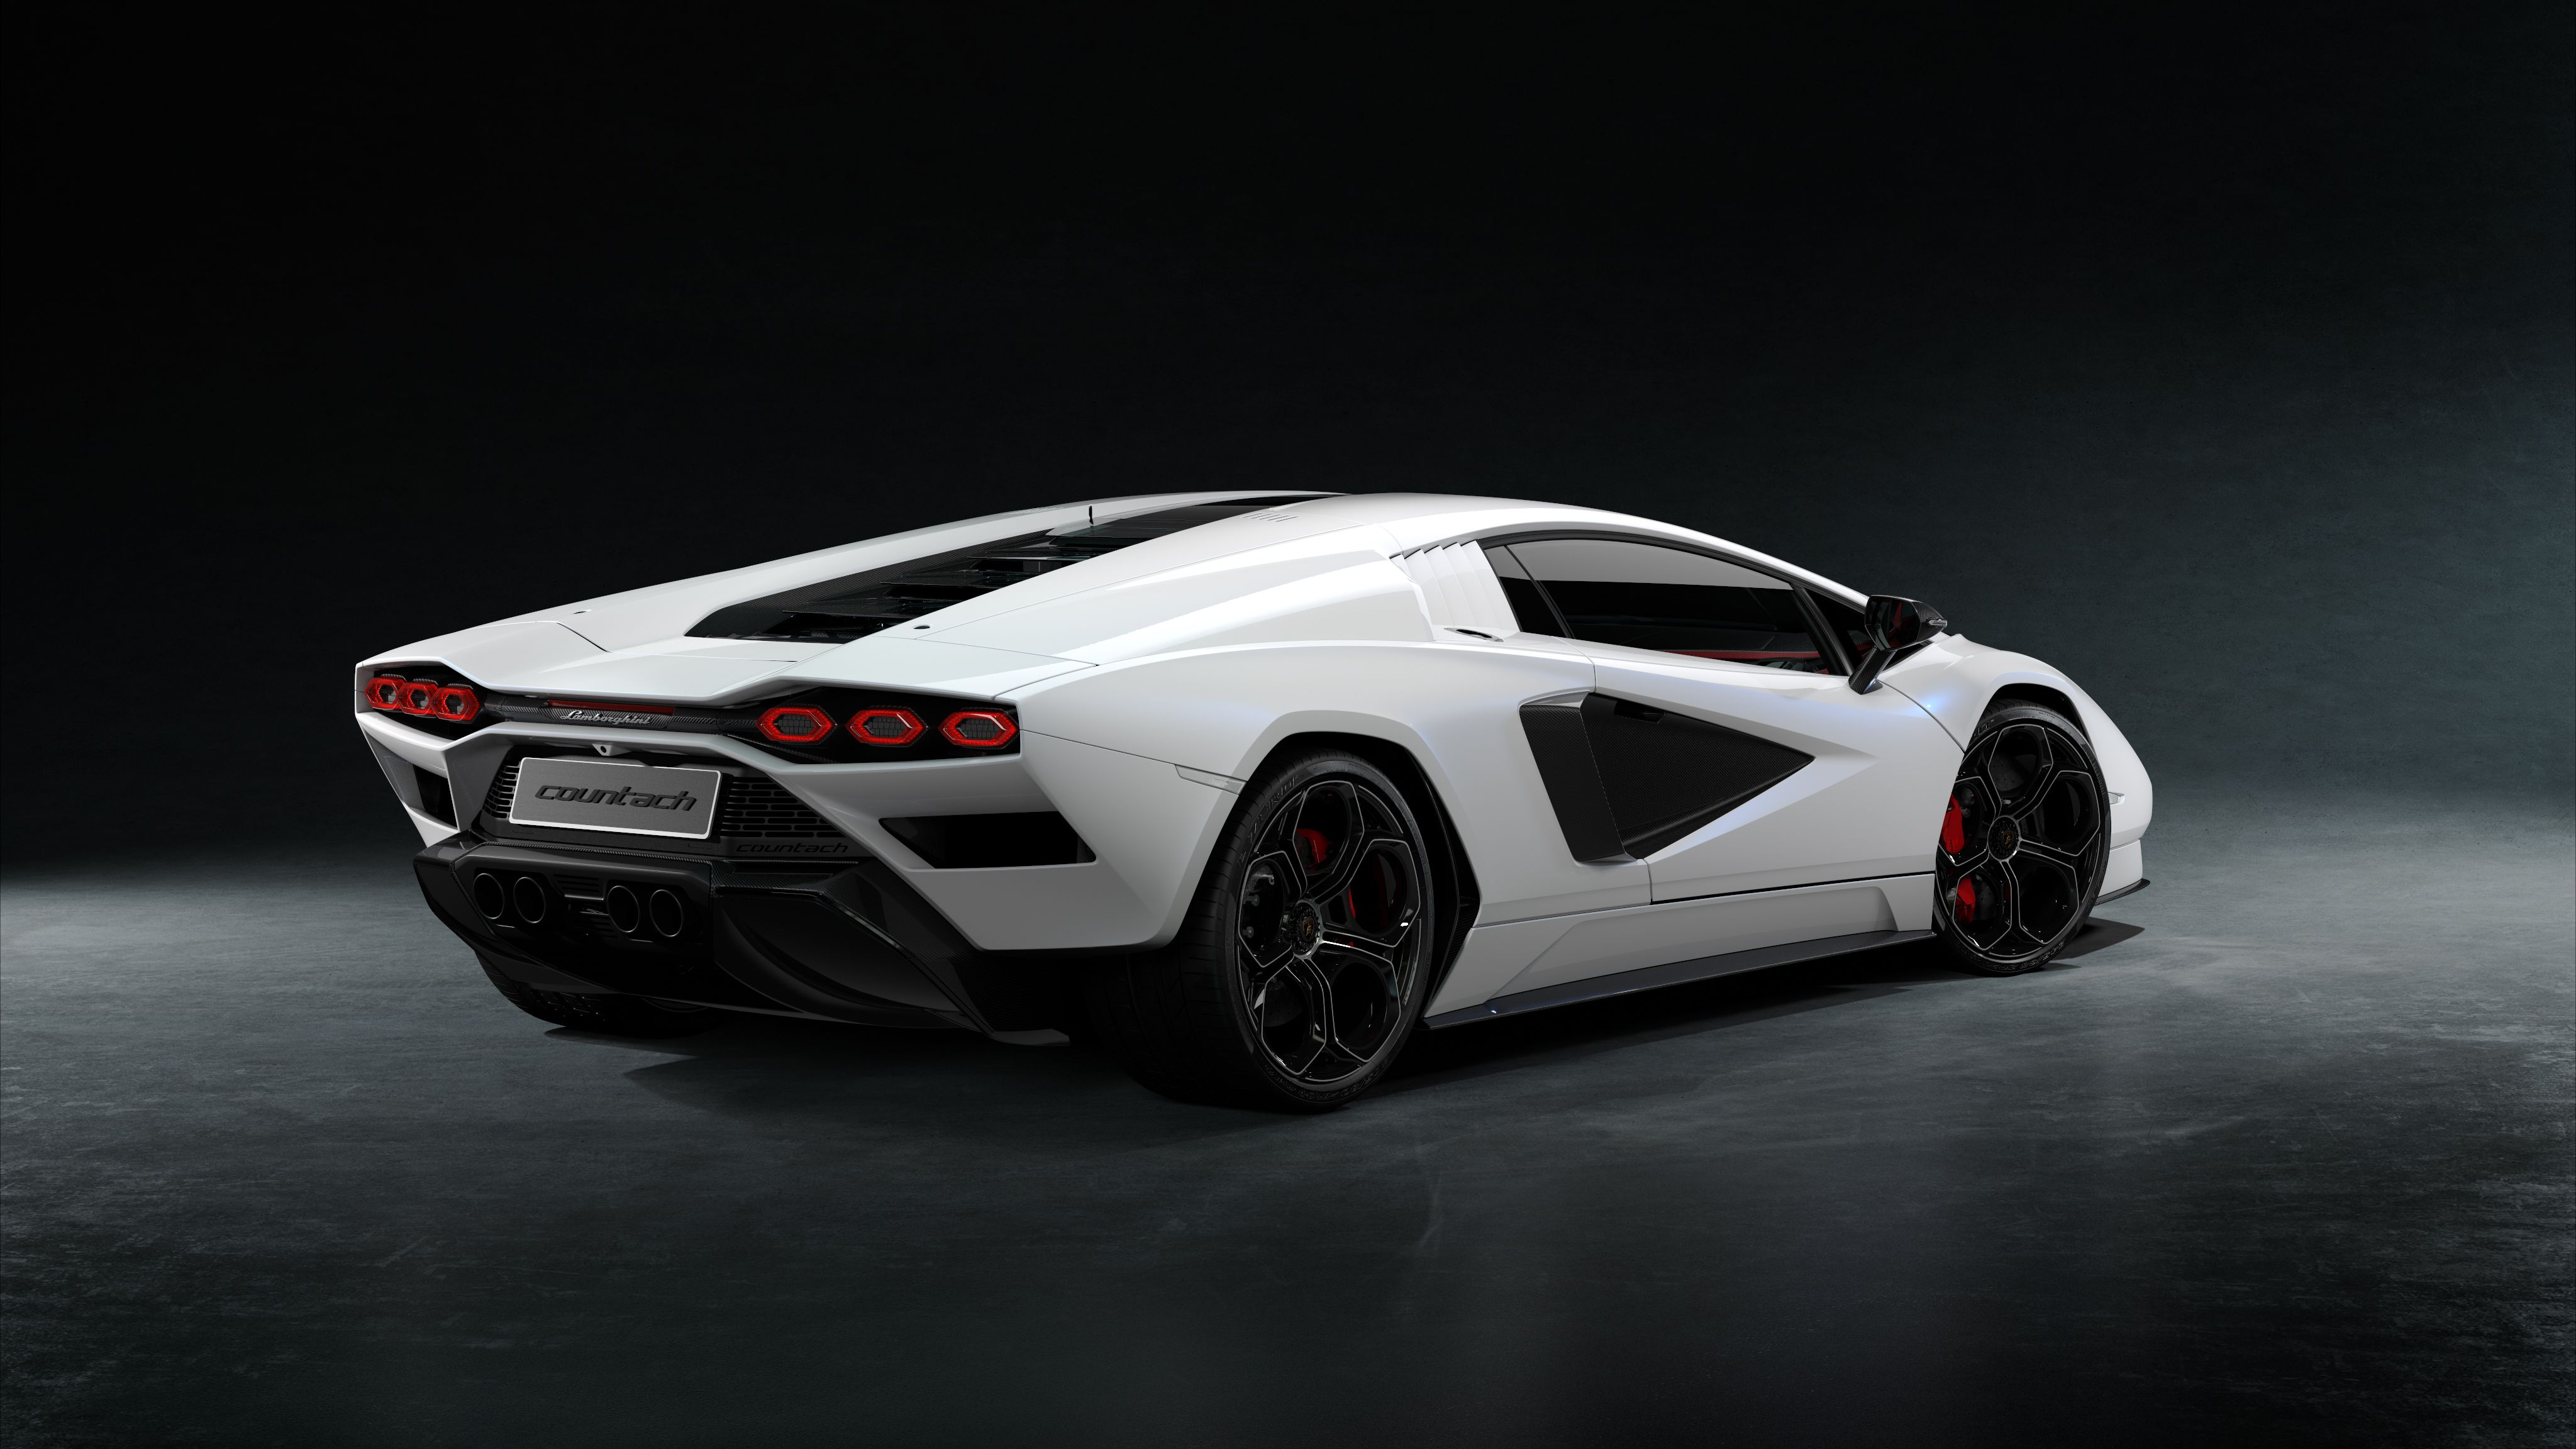
\includegraphics[width=\linewidth]{images/lambo.jpeg}
\end{center}

\vspace{1in}

\begin{center}
    Università di Bologna\\
    Campus di Cesena\\
    Facoltà di Ingegneria e Scienze Informatiche
\end{center}

\newpage

\mbox{}

\newpage

\tableofcontents

\newpage

\section{Analisi dei requisiti}
\subsection{Intervista}
La concessionaria desidera che vengano mantenuti in memoria i dati dei propri
clienti con nome, cognome, numero di telefono ed opzionalmente email. Per poter
acquistare una autovettura bisogna disporre del badge di iscrizione alla
concessionaria rinnovabile annualmente che identifica il cliente.\\
Oltre ai clienti iscritti alla concessionaria potrebbero venire in visita
persone comuni non iscritte delle quali non si ha interesse nel memorizzarle.
Considerando che non tutte le vetture in vendita sono presenti fisicamente nel
salone della concessionaria si richiede un sistema per la creazione di ordini
che possono includere più di una vettura. Ogni cliente possiede uno storico di
super car acquistate, utile alla azienda ai fini di marketing.\\
I dipendenti vengono distinti per nome, cognome, email aziendale e numero di
telefono aziendale e hanno uno storico delle proprie auto vendute. Inoltre, i
dipendenti, possono ottenere un bonus sullo stipendio se raggiungono un numero
minimo di vendite mensili, questo sistema incoraggia le vendite.\\
Le vetture del catalogo che andranno mantenute in memoria sono definite dal
codice di telaio, marca, modello, colore, unico segmento [Sport, Luxury,
SUV,...], cavalli potenza, prezzo, e colore. Una vettura può essere acquistata
da un solo cliente che ogni 2 anni potrà portarla nel officina della
concessionaria per manutenzione ordinaria, servizio gratuito esplicitato al
momento del ordine. Una autovettura può essere prodotta da un solo produttore
detto anche \textit{Casa Automobilista} identificato dal proprio nome, la quale
per lo stesso modello crea diversi restyling.\\
La super car può essere equipaggiata da optional differenti, i quali possono
essere prodotti da fornitori diversi. Ogni segmento possiede i propri optional
che alle volte vengono condivisi da più segmenti (ad esempio il Clima Automatico
o il Cambio Automatico sono optional presenti in ogni segmento a differenza del
Paraurti rinforzato che può essere montato solo su vetture di grandi dimensioni
presenti nei segmenti SUV ed OffRoad). Ogni optional è definito da una
descrizione, un codice prodotto e un livello di qualità di costruzione da 1 a
10.\\
Un cliente della concessionaria può eventualmente mettere in conto-vendita le
proprie autovetture ma solo nel caso rispettino gli standard qualitativi della
concessionaria, viene quindi fatta una valutazione da un professionista della
concessionaria che redige una scheda che descrive lo stato della vettura da
affiancare al contratto di conto-vendita. Il conto-vendita é composto da una
sola autovettura ed il prezzo è scelto dal proprietario. Nel contratto di
conto-vendita è presente una commissione che la concessionaria trattiene.

\subsection{Rilevamento delle ambiguità e analisi del intervista} 

Si procede con un analisi del testo frammentanta, analizzando parte per parte e
costruendo i relativi scheletri degli schemi E/R .

\subsubsection{Clienti}
\textbf{La concessionaria desidera che vengano mantenuti in memoria i dati dei propri
clienti con nome, cognome, numero di telefono ed opzionalmente email. Per poter
acquistare una autovettura bisogna disporre del badge di iscrizione alla
concessionaria rinnovabile annualmente che identifica il cliente.}

Si rileva che il cliente è un concetto fondamentale per la concessionaria e
viene identificato con un tesserino chiamato BADGE. Non è uno strumento
realmente utile alla concessionaria per la vendita, bensì è uno strumento di
marketing che vuole fidelizzare il cliente trasmettendo un senso di esclusività.
Il BADGE è unico ed appartene ad un solo proprietario che a sua volta ne può
avere uno solo. Il BADGE, inoltre, è rinnovabile annualmente quindi mantiene lo
stesso codice ma cambia la data di scadenza.

\begin{center}
    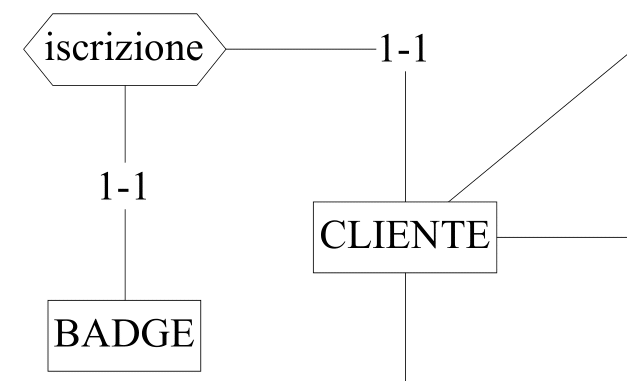
\includegraphics[width=\linewidth]{images/partialSchemes/cliente.png}
\end{center}

\subsubsection{Ordini}
\textbf{Oltre ai clienti iscritti alla concessionaria potrebbero venire in visita
persone comuni non iscritte delle quali non si ha interesse nel memorizzarle.
Considerando che non tutte le vetture in vendita sono presenti fisicamente nel
salone della concessionaria si richiede un sistema per la creazione di ordini
che possono includere più di una vettura. Ogni cliente possiede uno storico di
super car acquistate, utile alla azienda ai fini di marketing.}

Non c'é interesse nel memorizzare i dati di persone comuni in visita alla
concessionaria. Per quanto riguarda i clienti invece, si vuole mantenere uno
storico delle supercar acquistate e dare la possibilità di creare ordini che
possono includere più di una vettura. Viene quindi introdotta l'entità ORDINE
che rappresenta un contratto di acquisto. Lo storico delle supercar acquistate
da un cliente è utile alla concessionaria al fine di conoscere i gusti del
cliente e proporre nuovi modelli che gli potrebbero interessare.
Le supercar presenti nel database sono sia quelle facenti parte di un ordine che 
non, quindi la cardinalità da SUPERCAR ad ORDINE è 0:1.

\begin{center}
    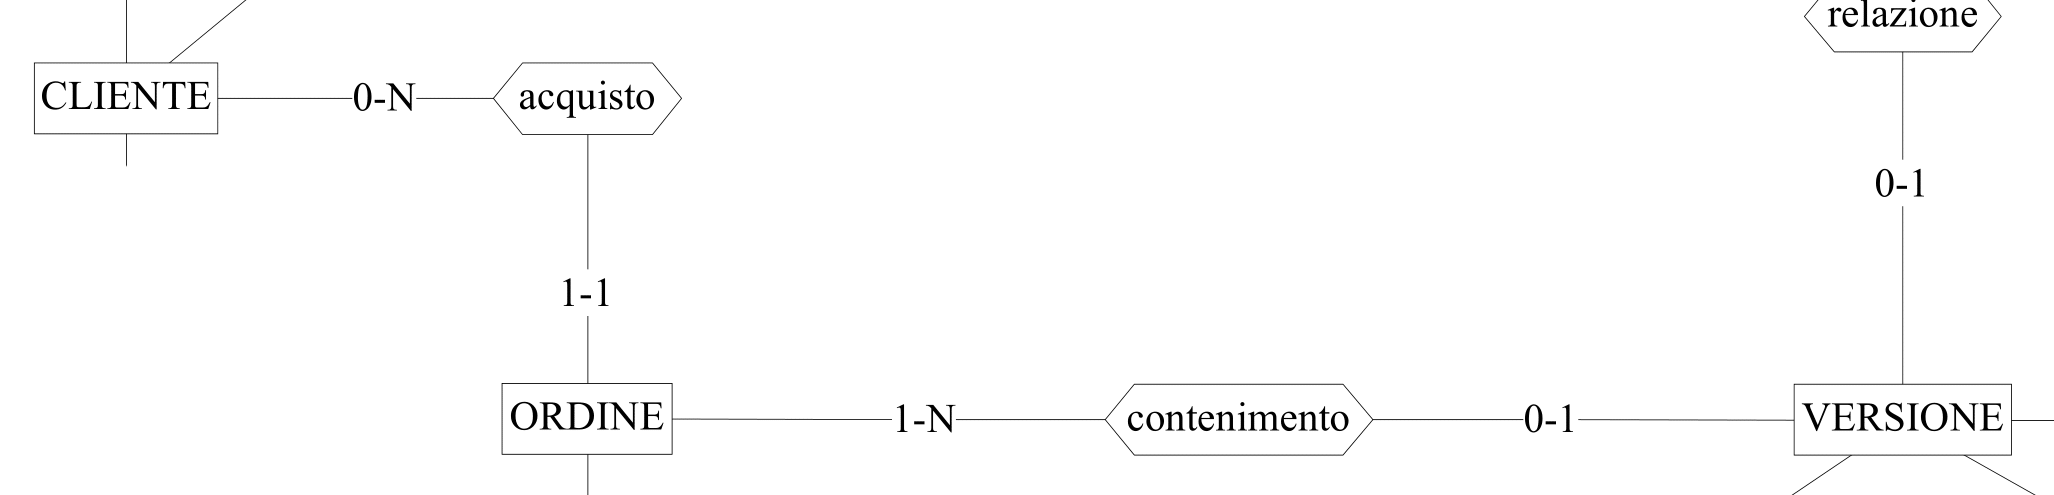
\includegraphics[width=\linewidth]{images/partialSchemes/ordine.png}
\end{center}

\subsubsection{Dipendenti}
\textbf{I dipendenti vengono distinti per nome, cognome, email aziendale e numero di
telefono aziendale e hanno uno storico delle proprie auto vendute. Inoltre, i
dipendenti, possono ottenere un bonus sullo stipendio se raggiungono un numero
minimo di vendite mensili, questo sistema incoraggia le vendite.}

A seguito di ulteriori indagini si rileva che ad identificare i dipendenti è la
mail aziendale, la quale è utile anche nella fase di log in nel applicativo.
Inoltre, viene tenuta memoria delle supercar vendute dai dipendenti per
valutarne il lavoro e per assegnare un bonus (mensile) nel caso abbiano superato
un obbiettivo di supercar vendute. Viene quindi introdotta l'entià STIPENDIO per
la memorizzazione opzionale del bonus. Per memorizzare lo storio delle vendite
invece si sfrutta l'entità ORDINE.

\begin{center}
    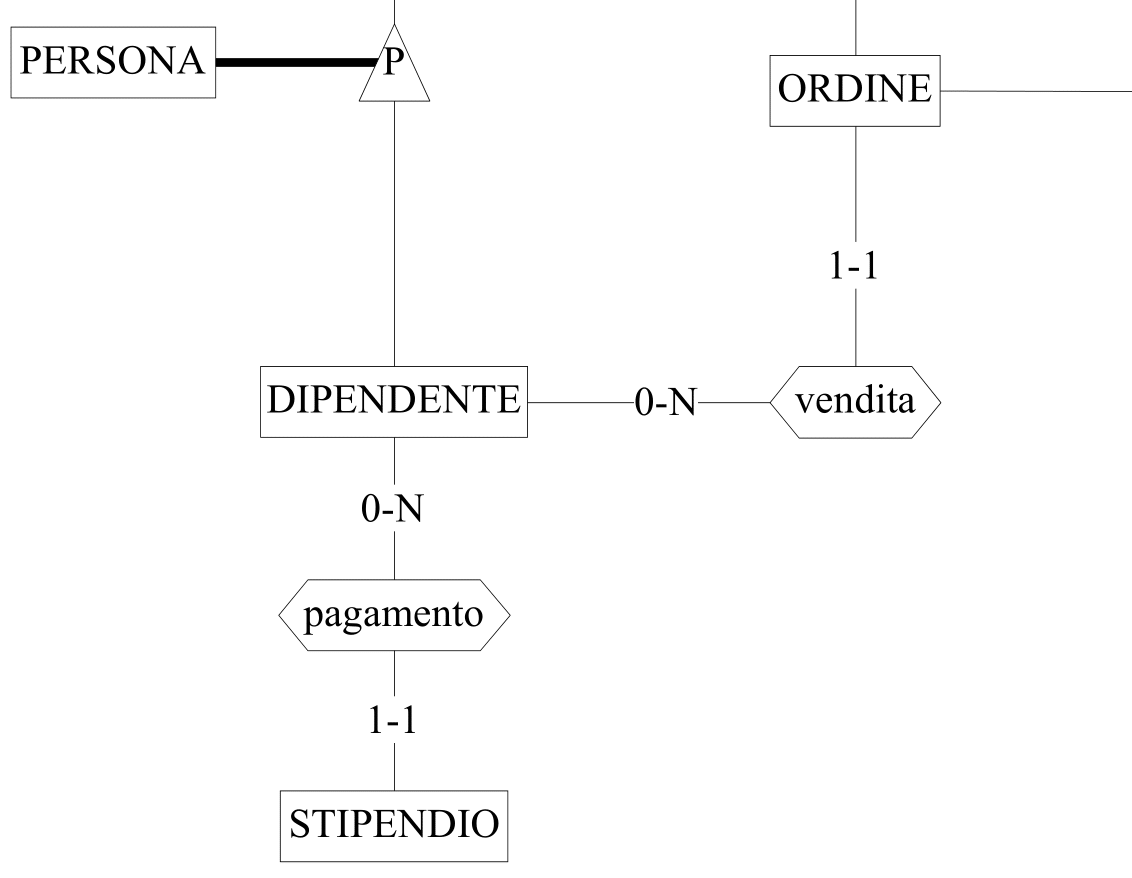
\includegraphics[width=\linewidth]{images/partialSchemes/dipendente.png}
\end{center}

\subsubsection{Supercar}
\textbf{Le vetture del catalogo che andranno mantenute in memoria sono definite
dal codice di telaio, marca, modello, colore, unico segmento [Sport, Luxury,
SUV,...], cavalli potenza, prezzo, e colore. Inoltre variano in base al
restyling. Una vettura può essere acquistata da un solo cliente che ogni 2 anni
potrà portarla nel officina della concessionaria per manutenzione ordinaria,
servizio gratuito esplicitato al momento del ordine. Una autovettura può essere
prodotta da un solo produttore detto anche \textit{Casa Automobilista}
identificato dal proprio nome, la quale per lo stesso modello crea diversi
restyling..}

Il codice del telaio è l'identificatore fondamentale di una qualsiasi vettura.
Il cliente, unico proprietario di una certa vettura acquistata, può portarla in
revisione dal officina della concessionaria ogni 2 anni gratuitamente.\\
Si pone particolare attenzione sul restylng di una supercar in quanto per un
certo modello possono essere prodotte diverse versioni. Viene quindi introdotta
l'entità VERSIONE che separa alcuni attributi dalla entità SUPERCAR. Il prezzo
ed il colore ad esempio variano in base alla versione della vettura quindi vanno
a caratterizzare una VERSIONE e non il modello; il primo per via delle leggi di
mercato, il secondo a causa di vetture a tiratura limitana che vengono prodotte
con colori particolari. Inoltre l'entità VERSIONE definisce anche istanze di
vetture che non hanno ricevuto un nuovo aggiornamento in quanto in termini
assoluti si trovano alla loro prima versione, ne segue che non esiste una
SUPERCAR senza almeno una VERSIONE. Per quanto riguarda il modello (sinominimo
di SUPERCAR), esso è prodotto da una CASA AUTOMOBILISTICA che attraverso il
proprio nome definisce la marca di una certa SUPERCAR.

\begin{center}
    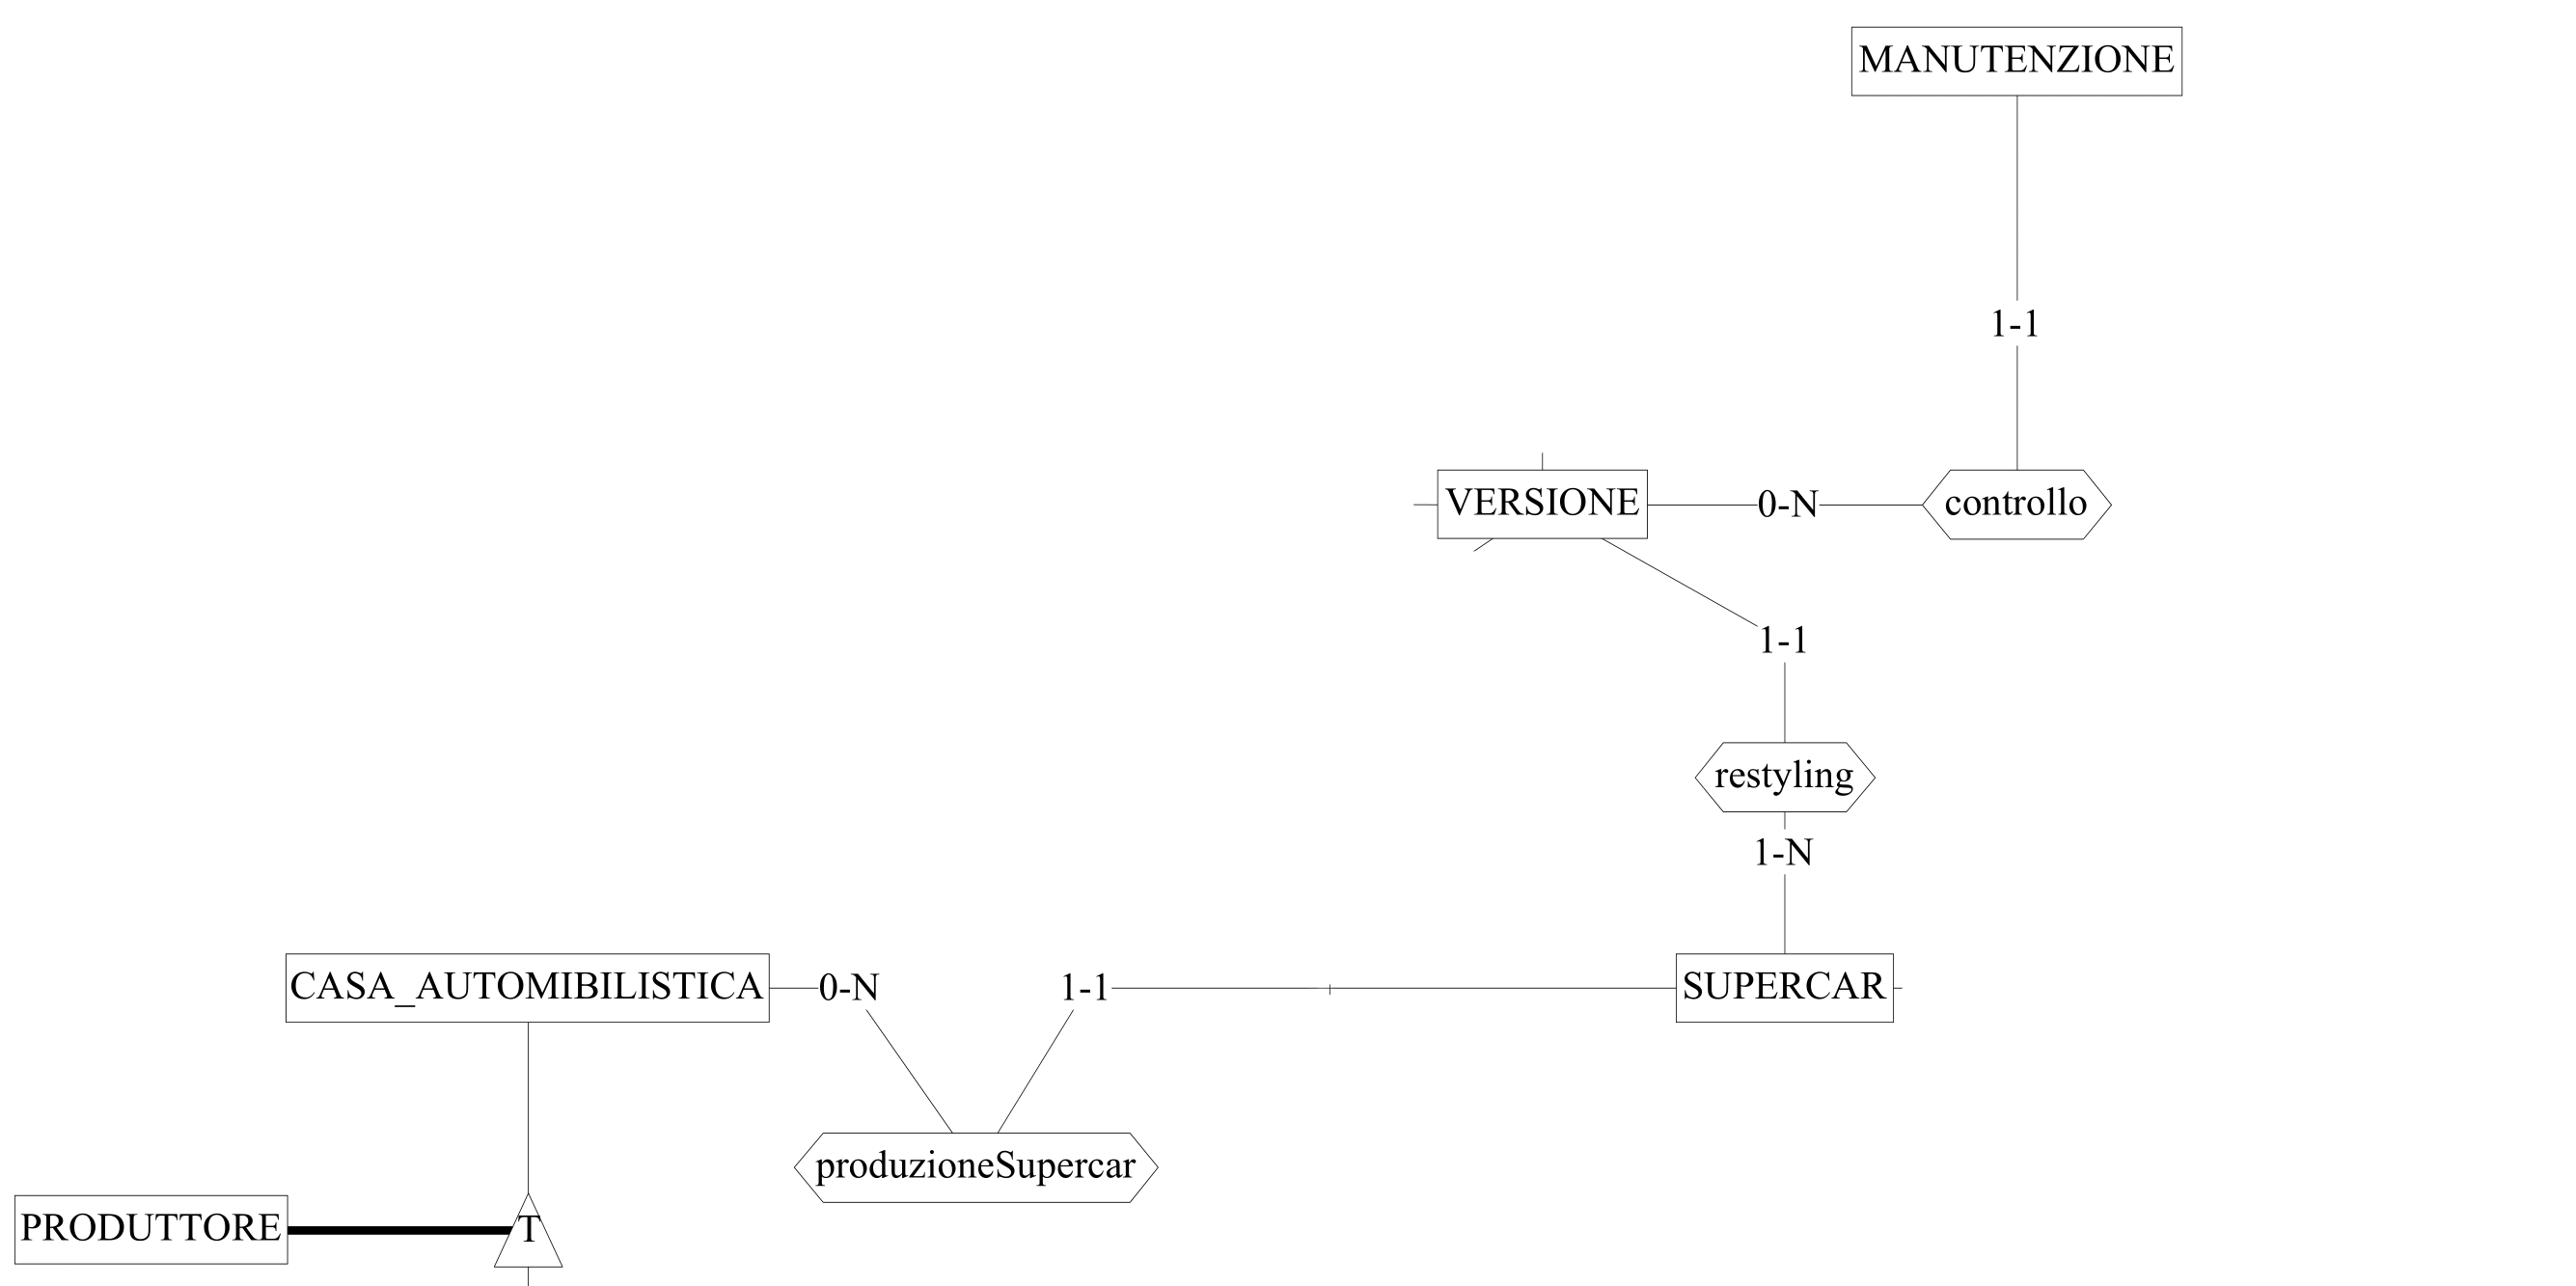
\includegraphics[width=\linewidth]{images/partialSchemes/versione.png}
\end{center}

\subsubsection{Optional e Produttore}
\textbf{La super car può essere equipaggiata da optional differenti, i quali
possono essere prodotti da fornitori diversi. Ogni segmento possiede i propri
optional che alle volte vengono condivisi da più segmenti (ad esempio il Clima
Automatico o il Cambio Automatico sono optional presenti in ogni segmento a
differenza del Paraurti rinforzato che può essere montato solo su vetture di
grandi dimensioni presenti nei segmenti SUV ed OffRoad). Ogni optional è
definito da una descrizione, un codice prodotto e un livello di qualità di
costruzione da 1 a 10.}

Si decide di trattare i segmenti come entità identificate dal proprio nome e
seguite da una descrizione. In generale un SEGMENTO è nient altro che il termine
tecnico per definire la categoria. Una supercar può equipaggiare optional
differenti, i quali devono appartenere allo stesso segmento della vettura. Gli
optional possono essere prodotti da diversi produttori, i quali possono anche
essere CASE AUTOMOBILISTICHE. Si introduce quindi una gerarchia Totale e
Sovrapposta che definisce i produttori di optional e le case automobilistiche.
Allo stesso modo delle VERSIONI, le quali essistono nel database senza far parte
di un orine, anche gli OPTIONAL esistono senza essere equipaggiati da una superacar.

\begin{center}
    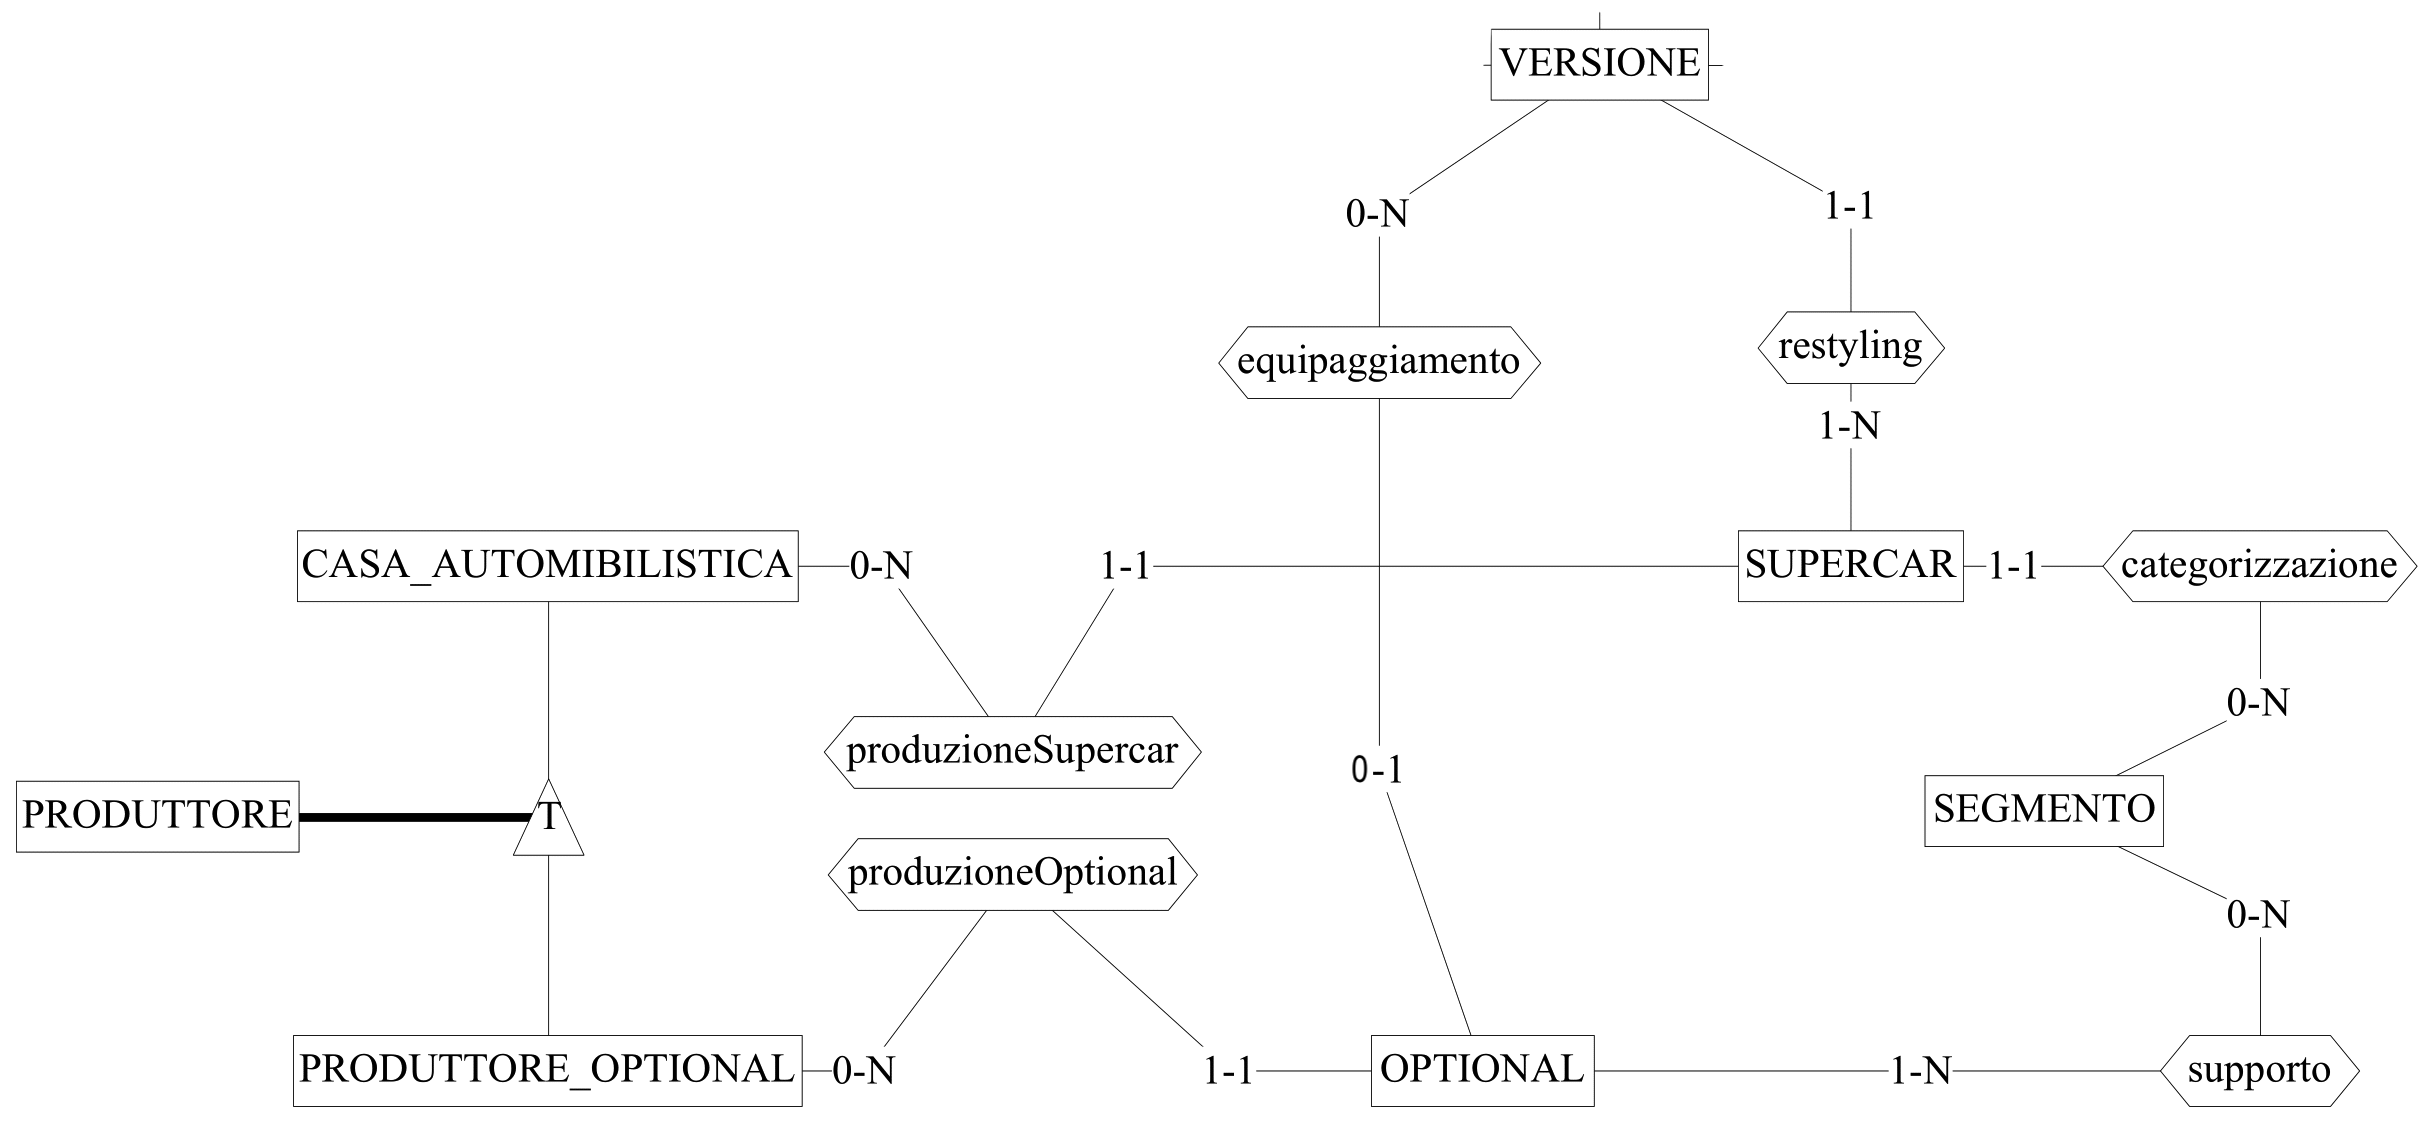
\includegraphics[width=\linewidth]{images/partialSchemes/optional.png}
\end{center}

\subsubsection{Conto-Vendita}
\textbf{Un cliente della concessionaria può eventualmente mettere in
\hyphenation{conto-vendita} le proprie autovetture ma solo nel caso rispettino
gli standard qualitativi della concessionaria, viene quindi fatta una
valutazione da un professionista della concessionaria che redige una scheda che
descrive lo stato della vettura da affiancare al contratto di
\hyphenation{conto-vendita}. Il \hyphenation{conto-vendita} é composto da una
sola autovettura ed il prezzo è scelto dal proprietario.\\ 
Nel contratto di \hyphenation{conto-vendita} è presente una commissione che la
concessionaria trattiene.}

Si rileva che il conto-vendita è un contratto di vendita che viene stipulato tra
concessionaria e CLIENTE. A seguito di ulteriori indagini si rileva che la
vettura in conto-vendita deve essere inserita nella struttura dati proprio come
una SUPERCAR comunemente venduta dalla concessionaria. Viene introdotta l'entità
CONTO-VENDITA che rappresenta il contratto alla quale viene affiancata la SCHEDA
DI VALUTAZIONE. E' importante precisare che non c’è un dipendente in particolare
ad occuparsi della conto-vendita ed è obbiettivo di tutti i dipendenti la più
rapida conclusione di questi contratti. In questo modo la vendita relativa ad
una vettura in conto-vendita non aumenta il numero di autovetture vendute dal
dipendente utili ad ottenere il bonus. La relazione tra CONTO-VENDITA e VERSIONE
esist in quanto il cliente può inserire in conto vendita una vettura già
presente nel database, nel caso non lo sia si procede al inserimento della
vettura per poi creare il contratto di conto vendita.

\begin{center}
    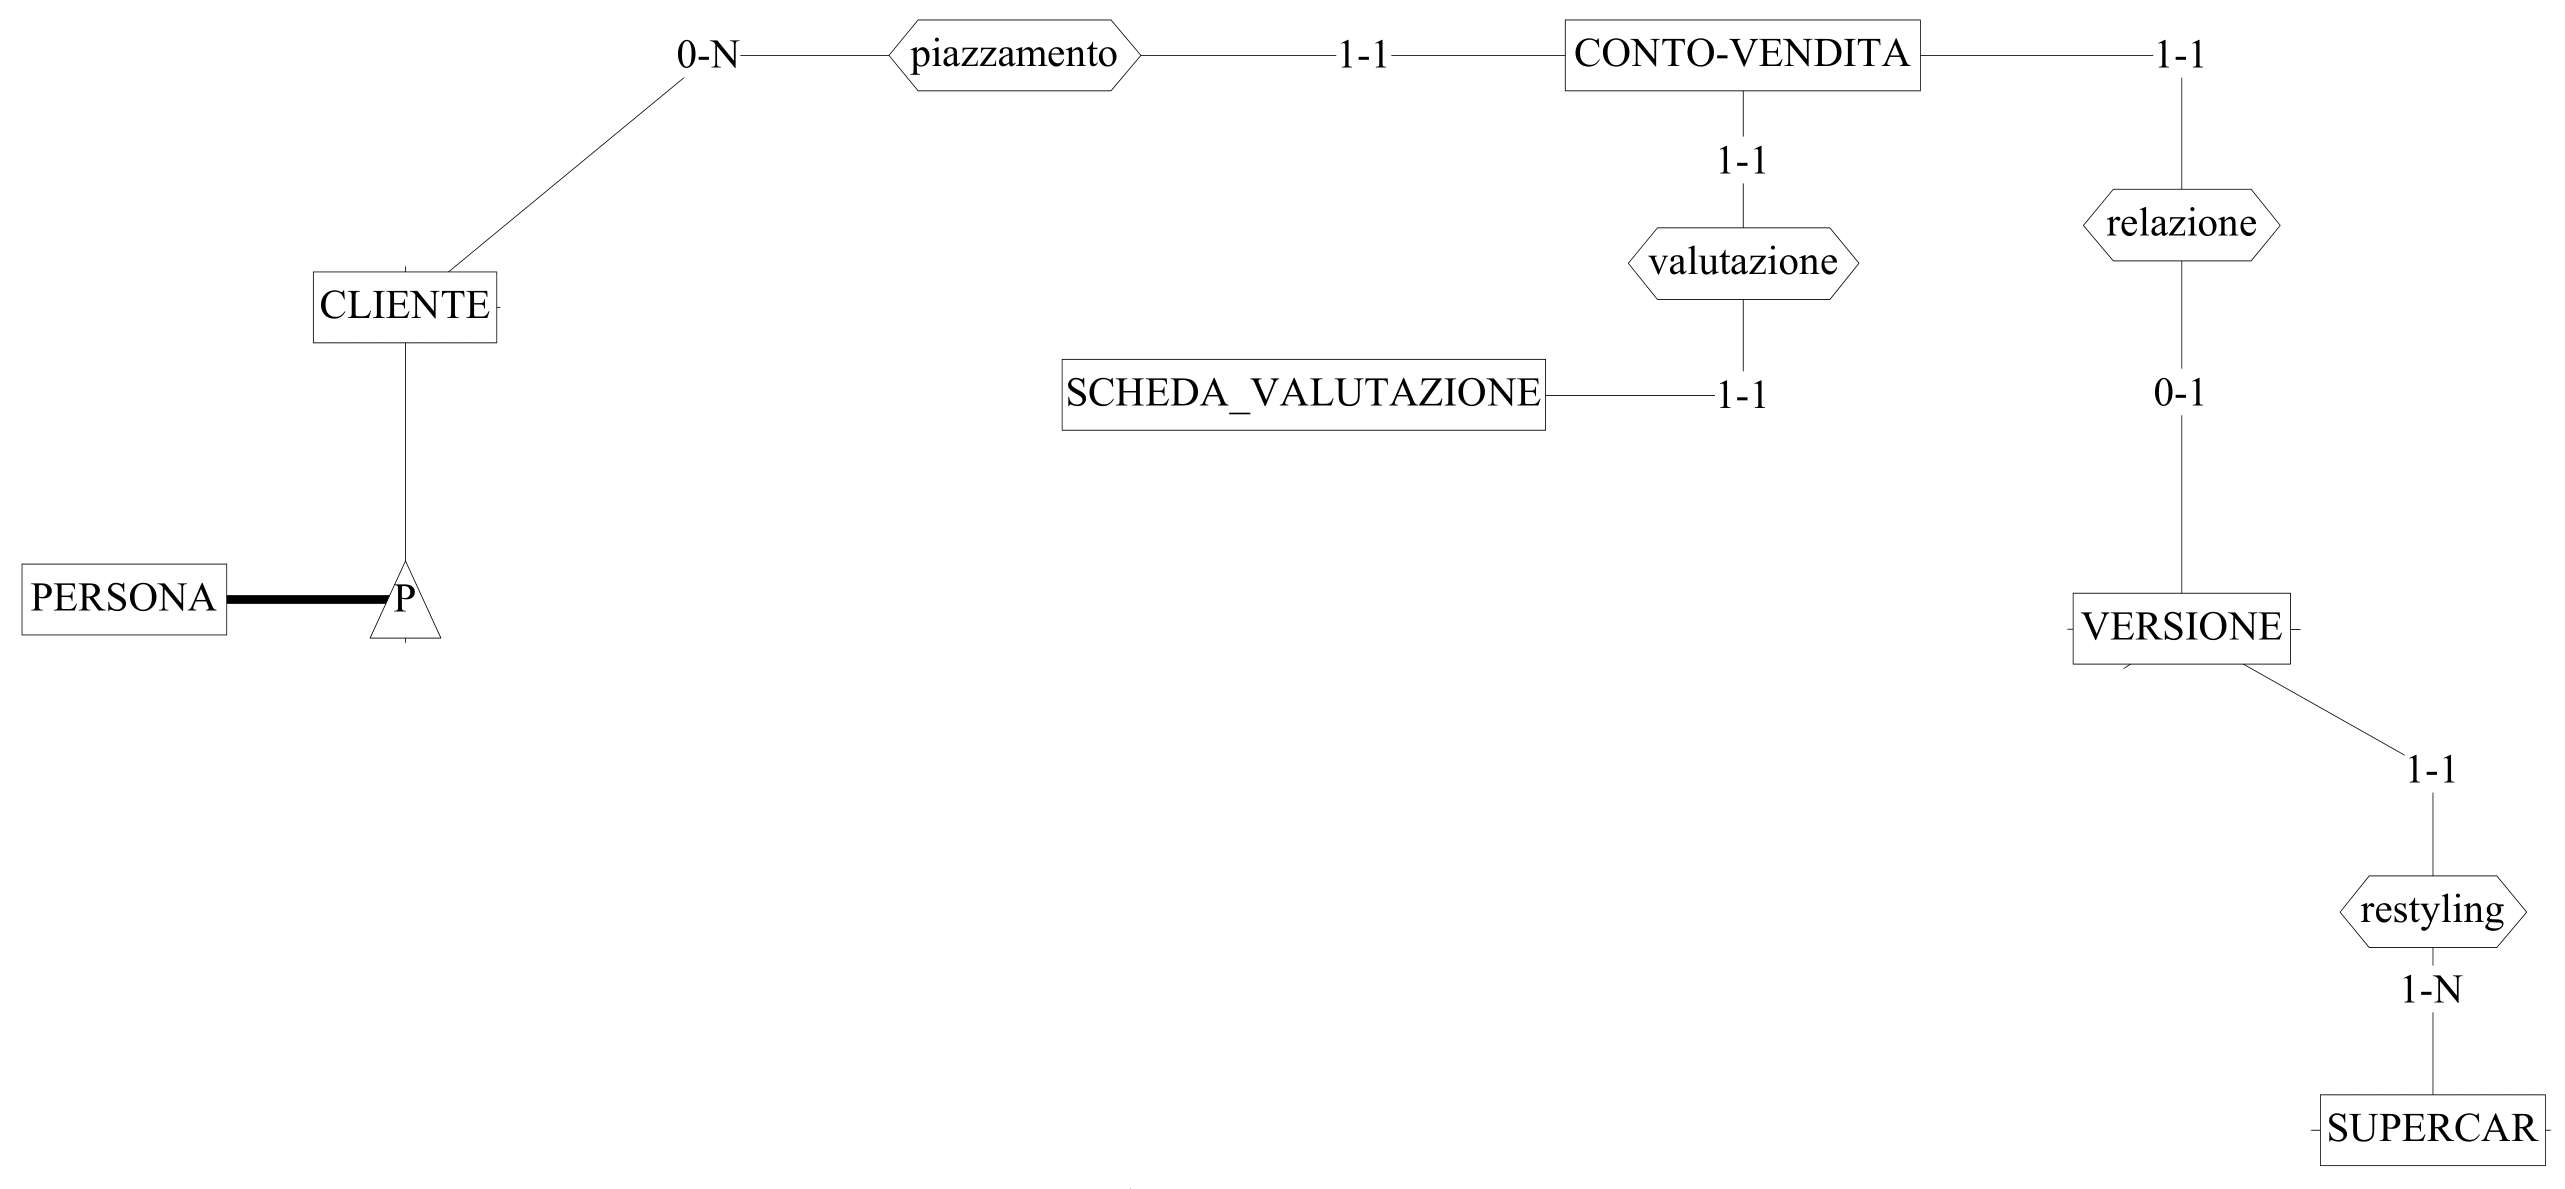
\includegraphics[width=\linewidth]{images/partialSchemes/contoVendita.png}
\end{center}

\newpage

\sloppy{\subsection{Definizione delle specifiche in linguaggio naturale
ed estrazione dei concetti principali}}

\renewcommand{\arraystretch}{1.5}

\begin{table}[htbp]
    \centering
    \small
    \rowcolors{2}{red!5!}{white}
    \begin{tabularx}{\linewidth}{l l X}
        \rowcolor{red!20!}
        \textbf{Numero} & \textbf{Nome} & \textbf{Concetto} \\
        1 & CLIENTE & compratore iscritto alla concessionaria \\
        2 & BADGE & tesserino utile al riconoscimento dei clienti \\
        3 & DIPENDENTE & venditore \\
        4 & ORDINE & contratto di acquisto di una o più vetture \\
        5 & STIPENDIO & paga mensile di un dipendente \\
        6 & CONTO-VENDITA & contratto di vendita di una vettura per conto
        di un cliente \\
        7 & SCHEDA VALUTAZIONE & descrive lo stato di una vettura in
        CONTO-VENDITA\\
        8 & VERSIONE & nuova versione di una supercar basata sullo stesso
        modello (es. Modello: Alfa Romeo Giulia, Versione: Edizione Anniversario) \\
        9 & SUPERCAR & modello prodotto da una Casa Automobilistica. Alle
        volte chiamata anche comunaente \textit{Modello} oppure \textit{Vettura}. \\
        10 & MANUTENZIONE & revisione di una super car (es. cambio del
        olio) \\
        11 & SEGMENTO & genere/tipologia/categoria di supercar (es. Sport, SUV, Berlina, OffRoad,..)\\
        12 & OPTIONAL & dispositivo che una vettura può equipaggiare
        opzionalmente \\
        13 & CASA AUTOMOBILISTICA & azienda produttrice di autovetture \\
        14 & PRODUTTORE OPTIONAL & azienda produttrice di optional \\
    \end{tabularx}
    \label{tab:tabella_linguaggio}
\end{table}

\section{Progettazione Concettuale}

\subsection{Schema scheletro assemblato}

\begin{center}
    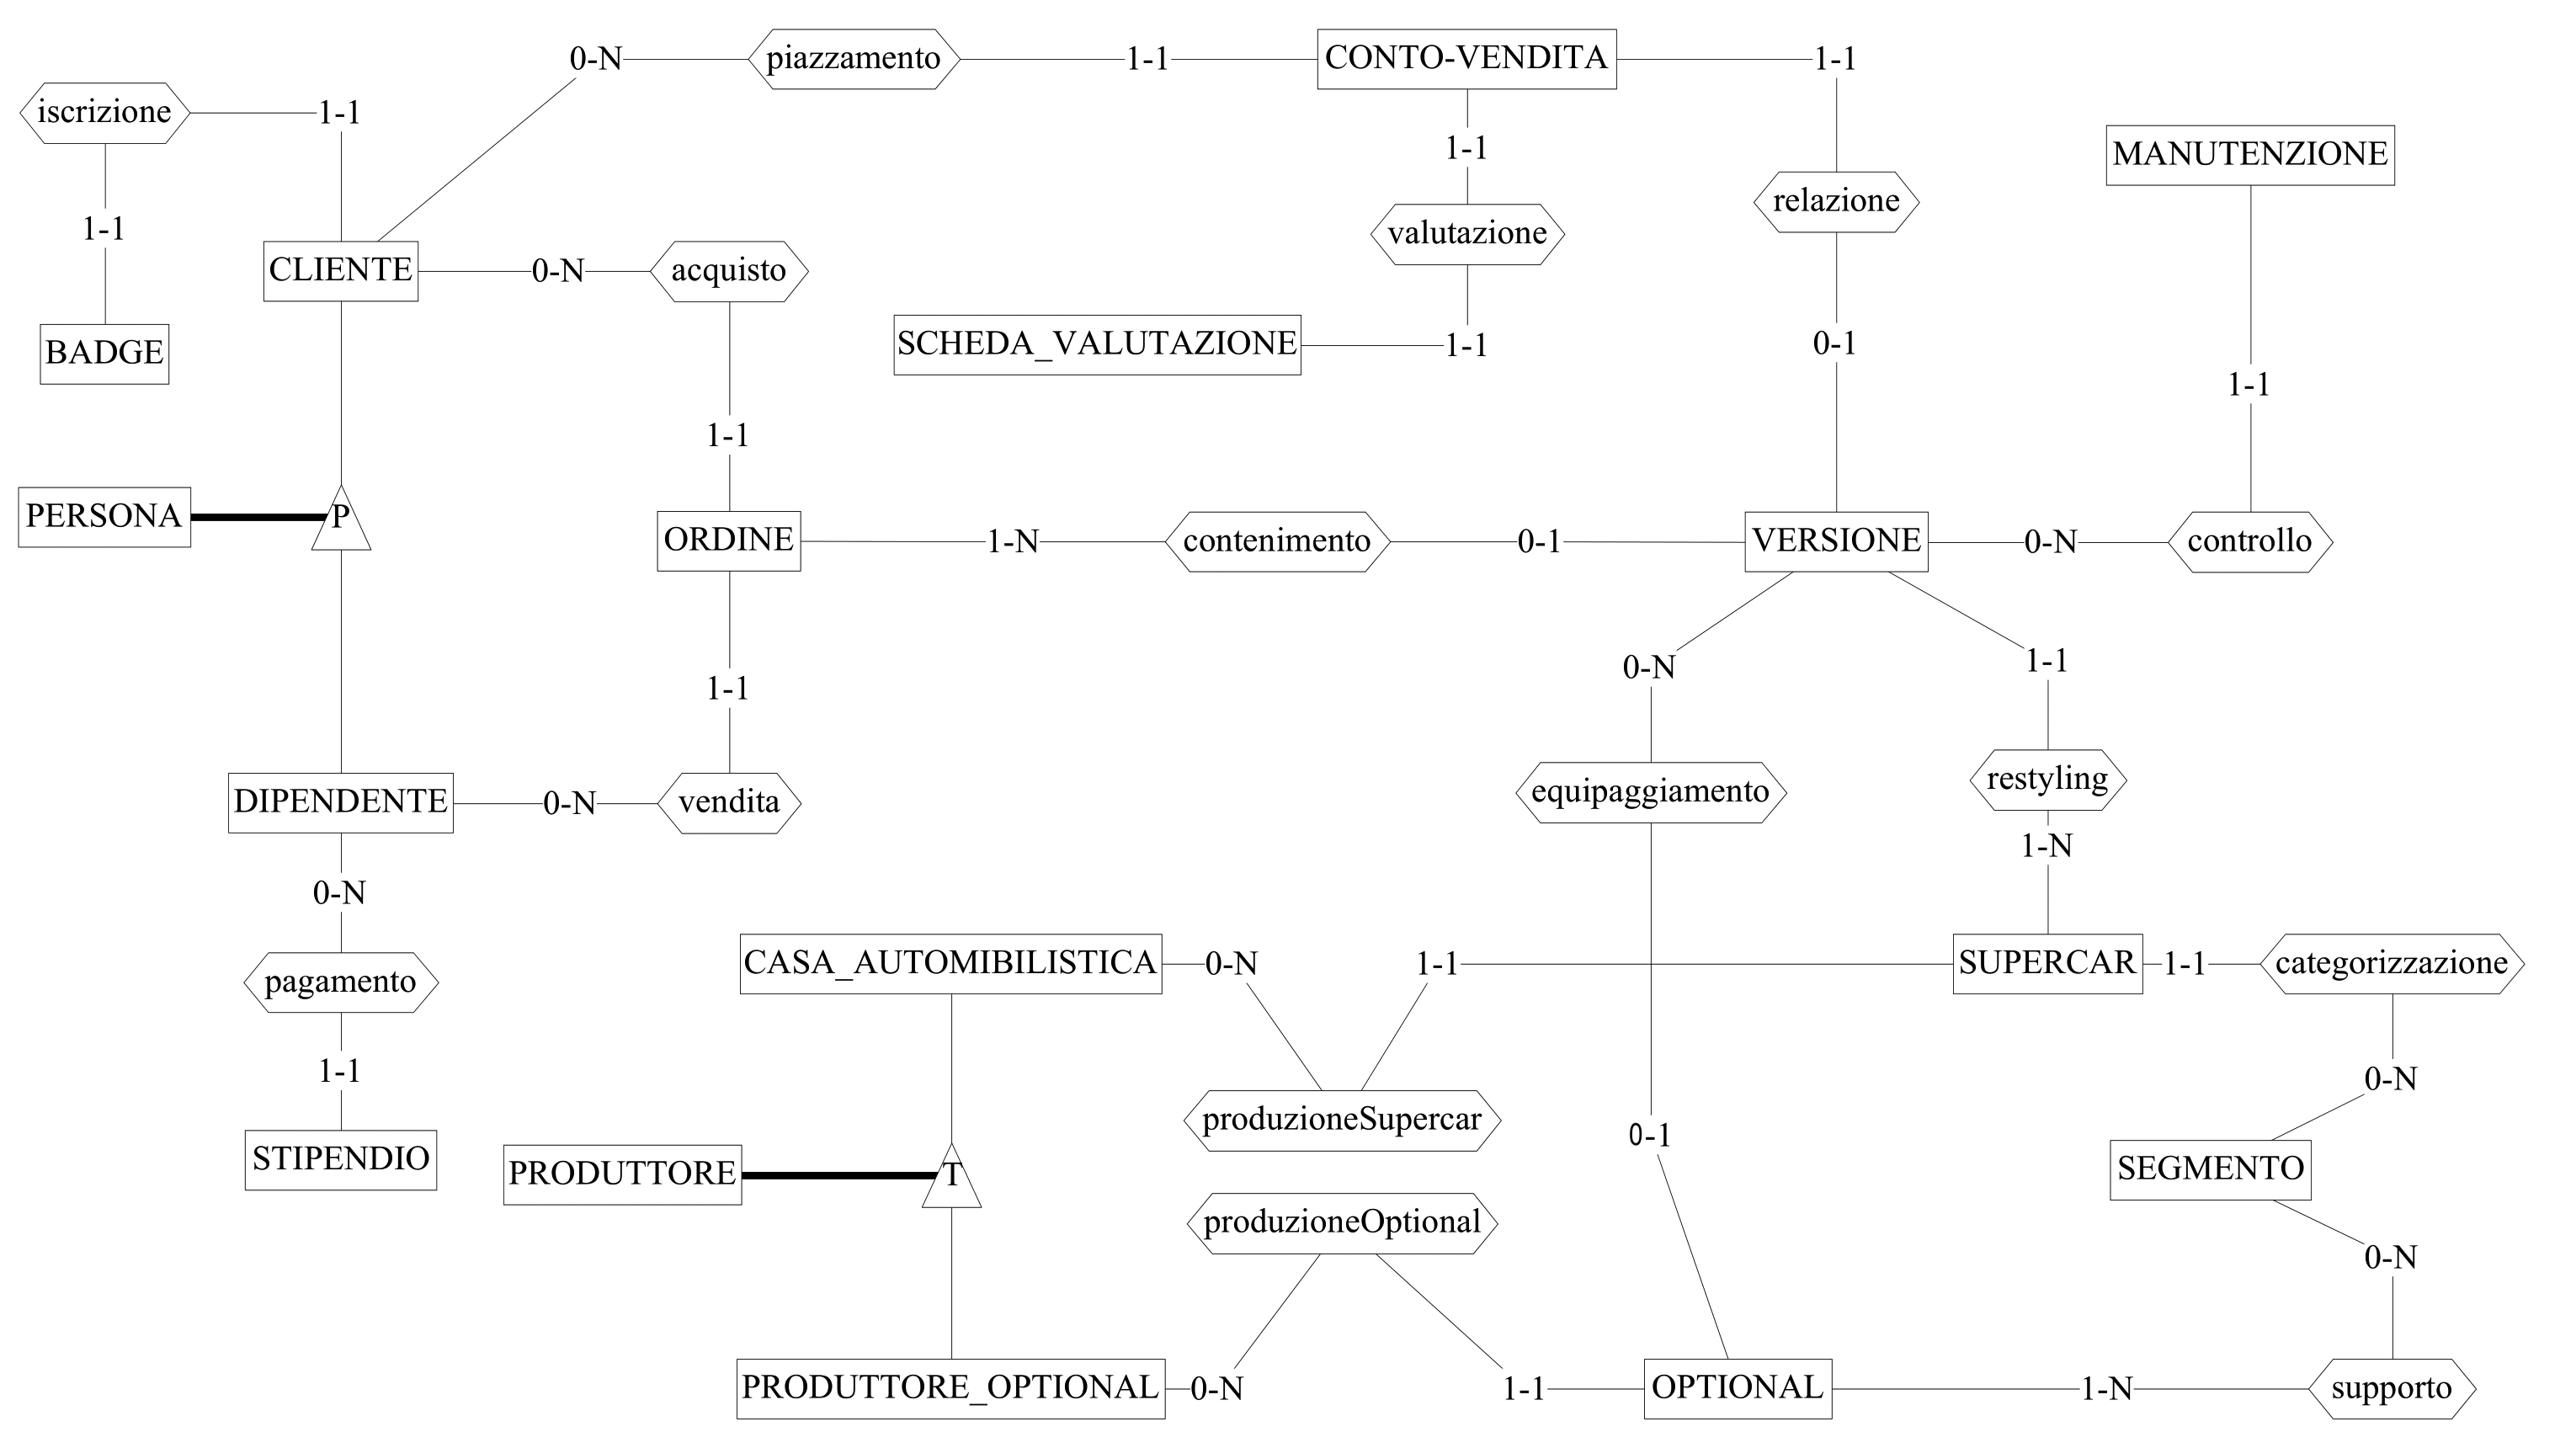
\includegraphics[scale=0.60, angle=90]{images/fullSchemes/scheletro.png}
\end{center}

\newpage

\subsection{Schema concettuale finale}
\begin{center}
    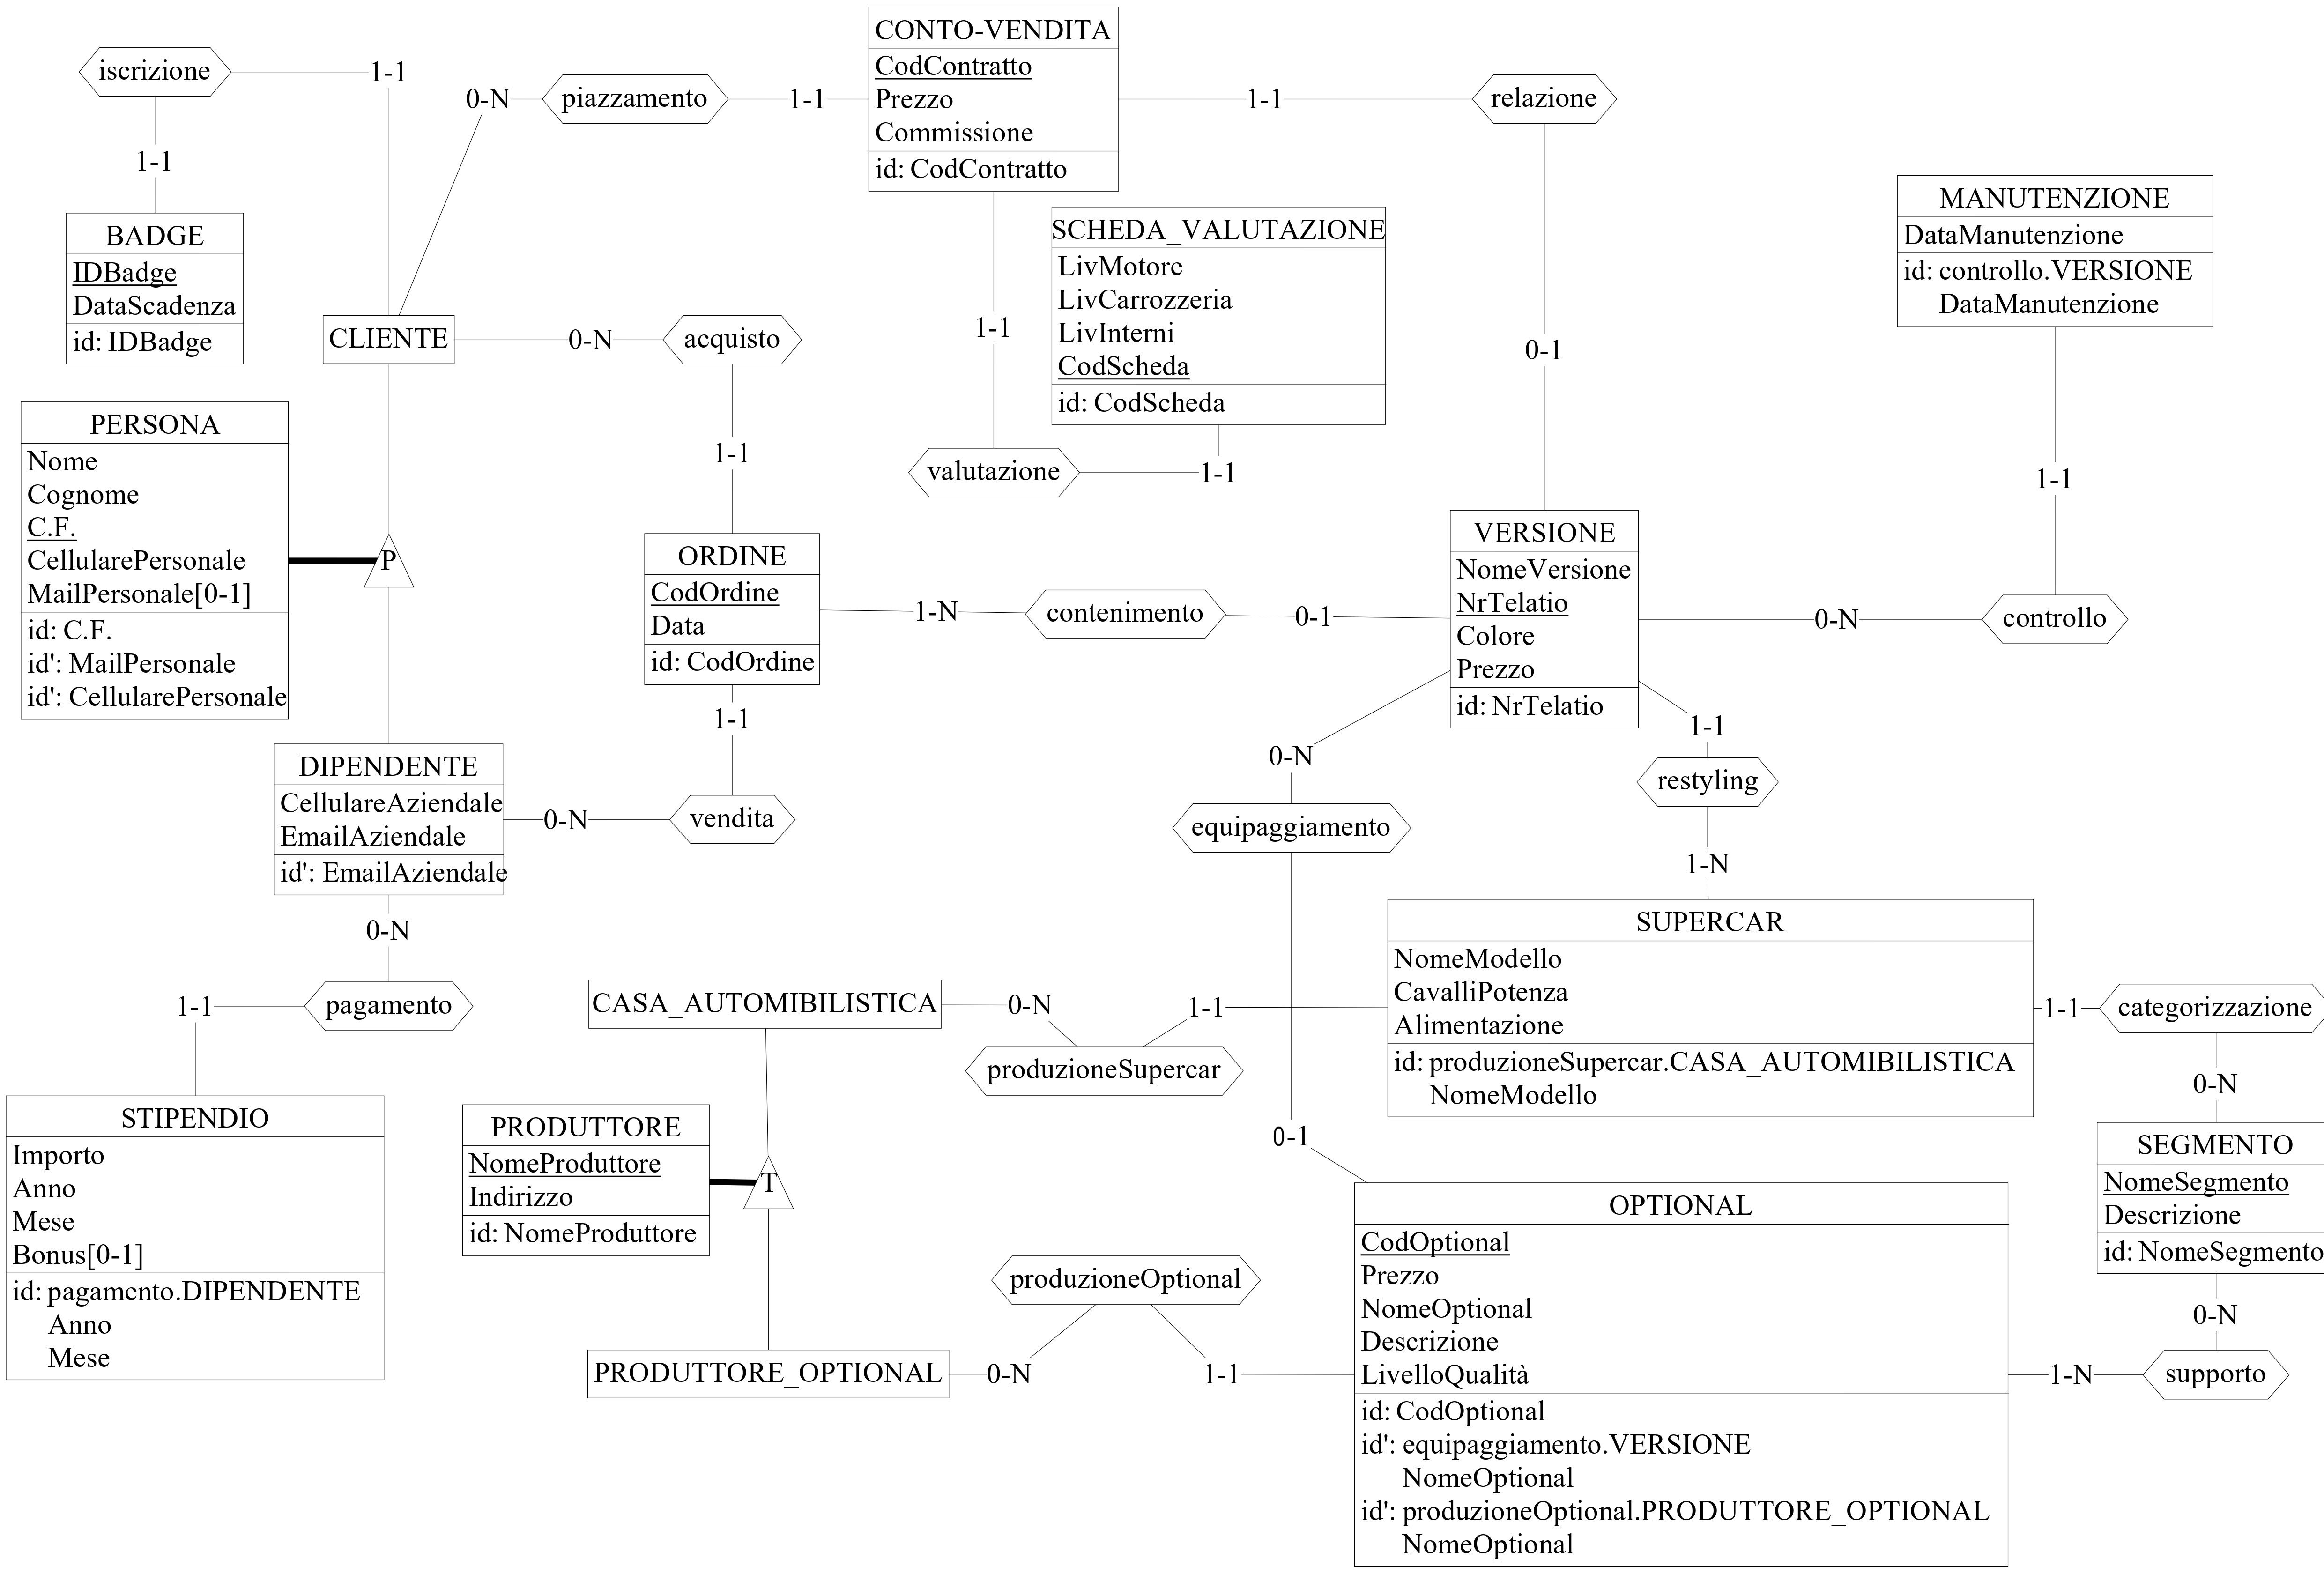
\includegraphics[height=\linewidth, angle=90]{images/fullSchemes/finale.jpeg}
\end{center}

\newpage

\section{Progettazione Logica}

\subsection{Stima del volume dei dati}

\subsubsection*{Accorpamento di Entità}

Le relazioni CLIENTE - BADGE ed CONTOVENDITA - SCHEDA VALUTAZIONE sono
state accorpate in quanto si tratta di relazioni 1:1 e non si
prospettano variziani future delle Entità BADGE ed SCHEDA
VALUTAZIONE. Il BADGE è stato accorpato alla entità CLIENTE mentre
la SCHEDA VALUTAZIONE è stata accorpata nel entità CONTOVENDITA.

\begin{center}
    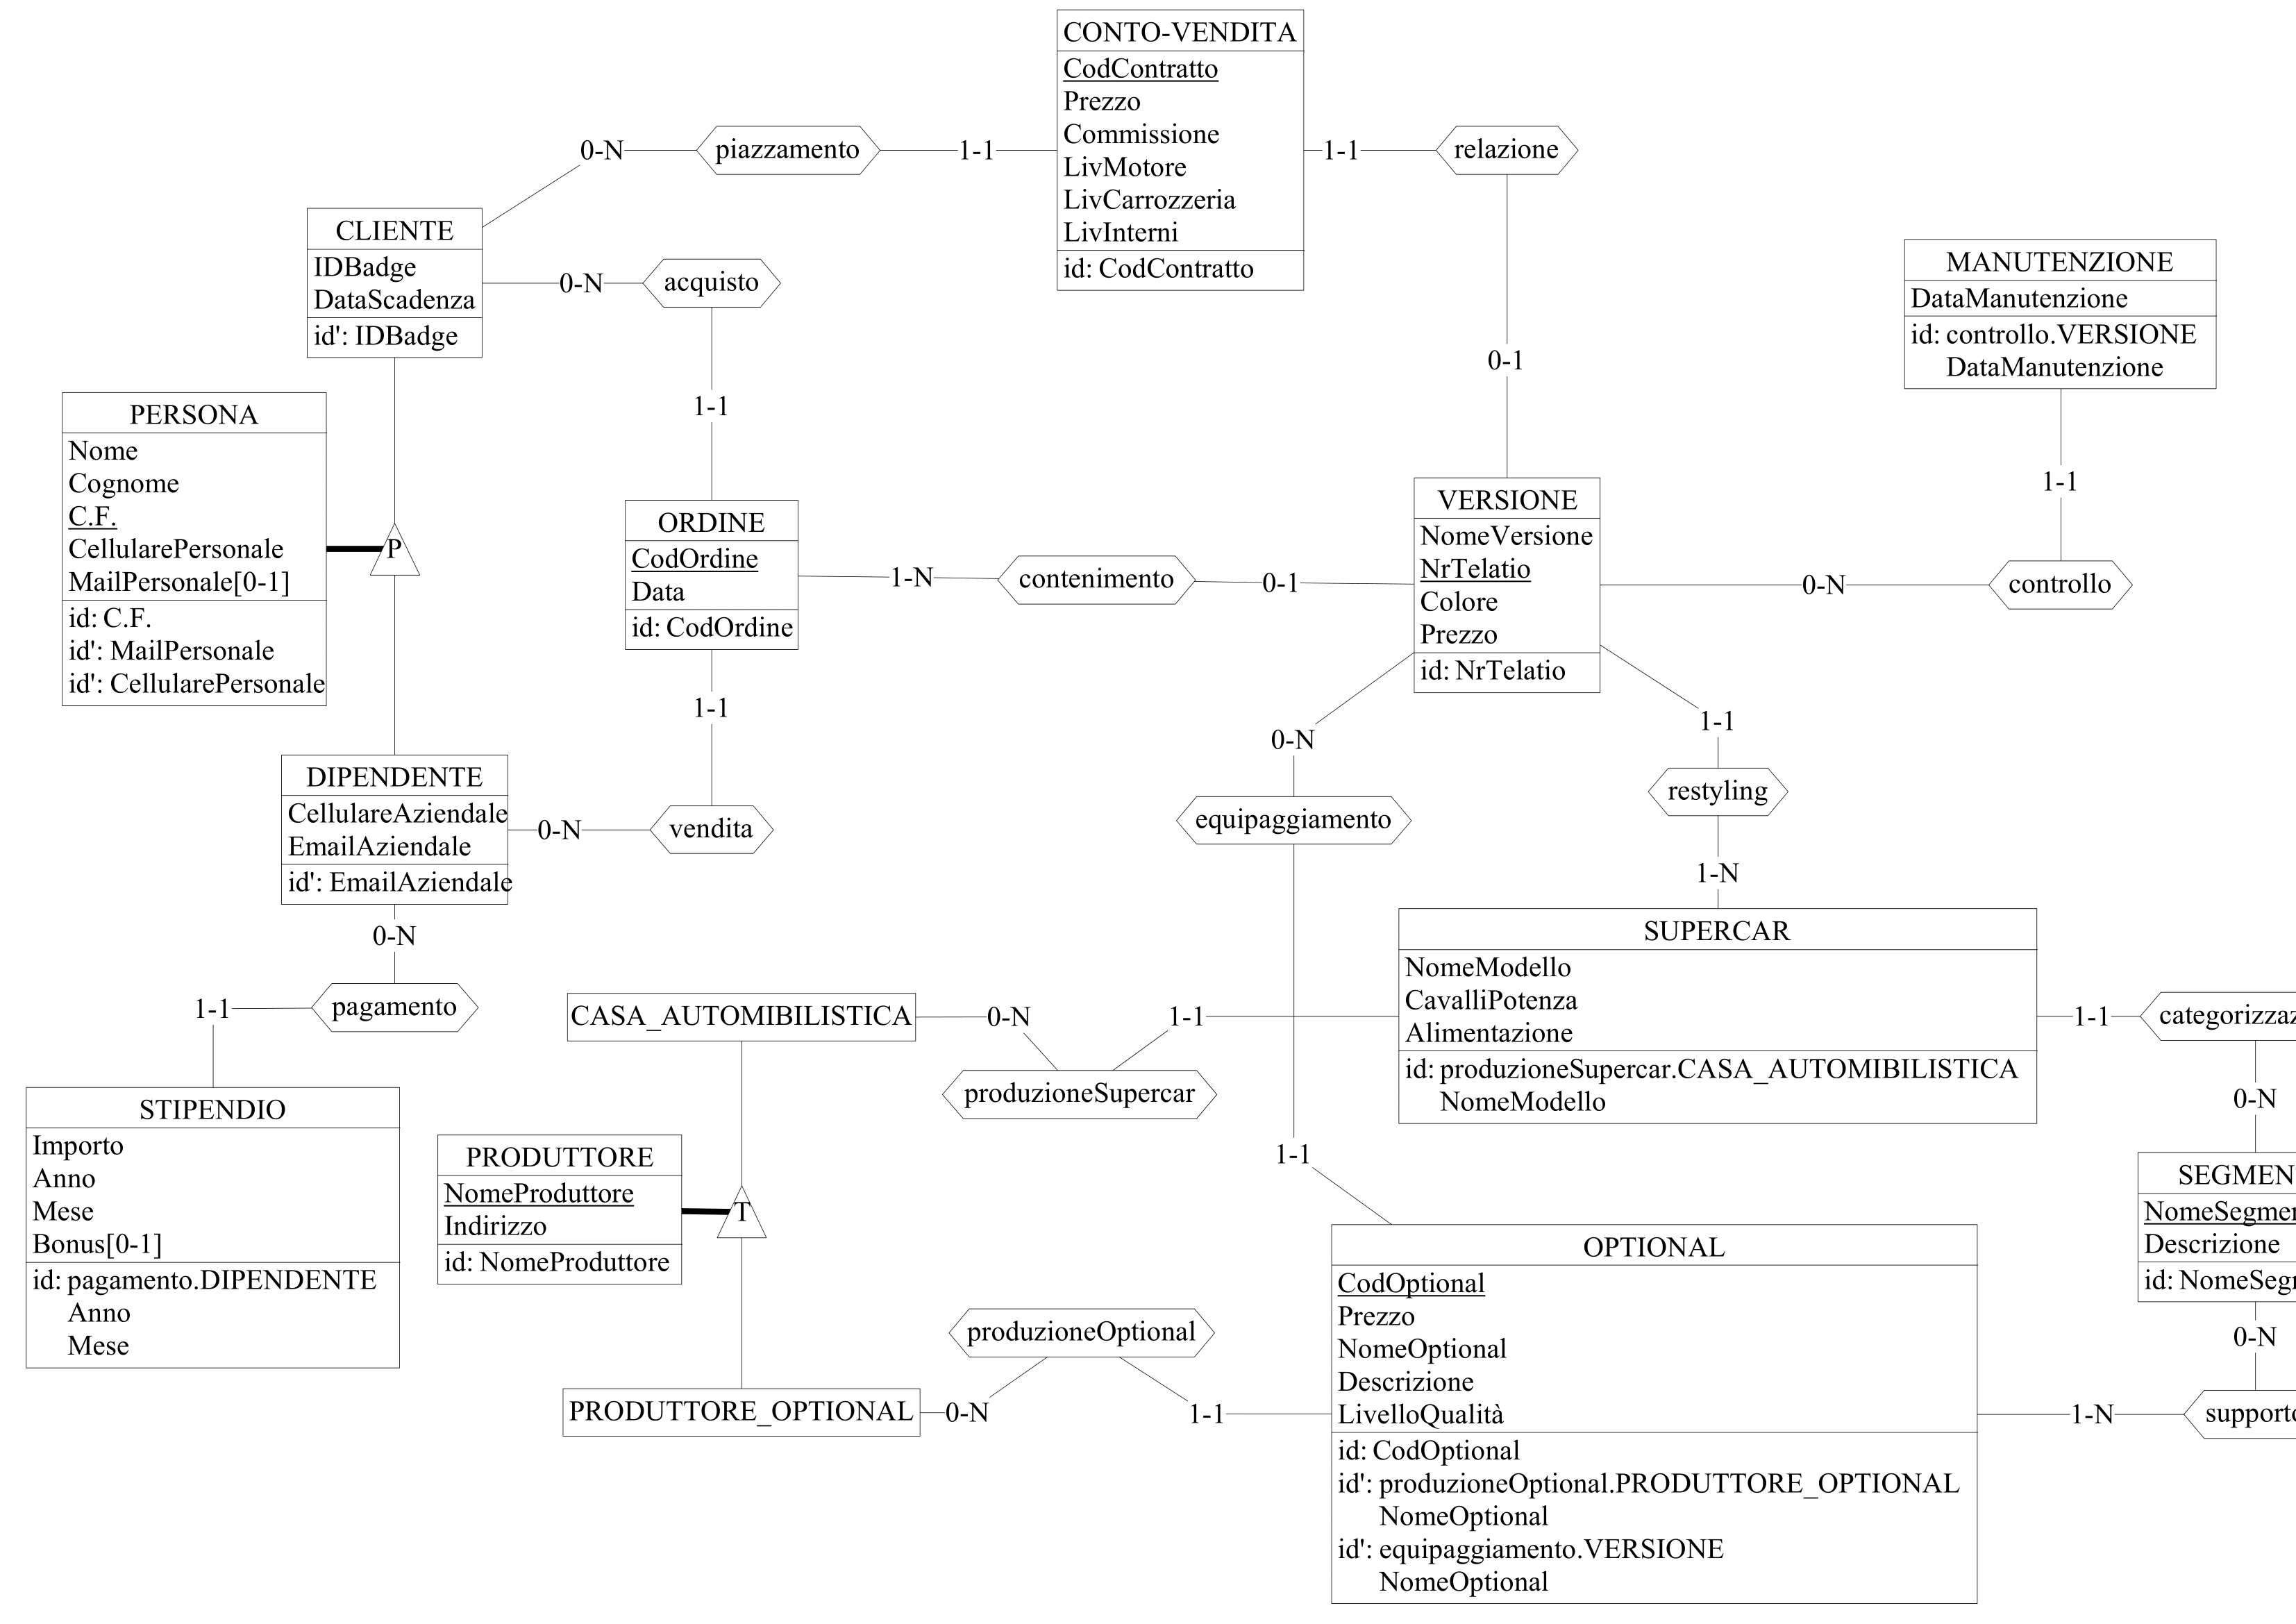
\includegraphics[scale=0.48, angle=90]{images/fullSchemes/finalAccorpamenti.png}
\end{center}

Di seguito la stima di dati valutata ad un anno dalla apertura della
concessionaria nel mercato di una città di grande dimensioni (es. Milano). 

\begin{table}[htbp]
    \centering
    \small
    \rowcolors{2}{red!5!}{white}
    \begin{tabularx}{\textwidth}{c l c X }
        \rowcolor{red!20!}
        \textbf{Tipo} & \textbf{Concetto} & \textbf{Volume} & \textbf{Nota}\\
        E & CLIENTE & 400 & \\
        E & DIPENDENTE & 30 & \\
        E & ORDINE & 800 & Si stimano mediamente 2 ordine a cliente. \\
        E & STIPENDIO & 390 & Mediamente ci sono 13 stipendi per dipendente. \\
        E & CONTO-VENDITA & 20 & \\
        E & VERSIONE & 1200 & In media in un ordine troviamo 1 oppure 2 vetture.
        \\
        E & MANUTENZIONE & 10 & Manutenzioni straordinarie dovute a difetti
                                lievi dovuti al trasporto. Le manutenzione
                                ordinarie non avevano modo di presentarsi ad un
                                anno dal apertura della concessioanria. \\
        E & SUPERCAR & 900 & Questo valore non è riferito solo alle supercar
                                rilasciate dalle case produttrici nel ultimo
                                anno ma anche di vetture di anni passati che a
                                loro volta hanno diverse versioni. \\
        
        E & SEGMENTO & 7 & Coupè, Hypercar, Berlina di Lusso, Berlina compatta,
        SUV, OffRoad, Sportiva \\
        R & Supporto & 1250 & Mediamente per ogni segmento ci sono un numero
                                considerevole di optional ma trattandosi di
                                vetture particolarmente lussuose il numero si
                                riduce in favore della qualità. \\
        E & OPTIONAL & 10'000 & \\
        E & CASA AUTOMOBILISTICA & 100 & \\
        E & PRODUTTORE OPTIONAL & 300 & \\  
        
    \end{tabularx}
    \label{tab:volume_table}
\end{table}

\newpage

\subsection{Descrizione delle operazioni principali e stima della loro frequenza}

Le seguenti operazioni vanno a descrivere il comportamento di un dipendente tipo
(ad eccezione delle numero 6 e 9) della concessionaria. In parte sono operazioni
comuni di vendita, altre di rilevazione statistica al fine di analizzare il
mercato e preformare al meglio nelle vendite. 

\begin{table}[htbp]
    \centering
    \small
    \rowcolors{2}{red!5!}{white}
    \begin{tabularx}{\linewidth}{c X c}
      \rowcolor{red!20!}
      \textbf{Codice} & \textbf{Operazione} & \textbf{Frequenza} \\
      1 & Log In di un dipendente & 900 al mese \\
      2 & Inserimento di un nuovo cliente & 33 al mese \\
      3 & Visualizza le vetture acquistate da un cliente in un certo periodo in
      ordine crescente di data & 14 al mese \\
      4 & Visualizza gli optional di una certa azienda & 20 al mese \\
      5 & Inserimento di un nuovo ordine & 66 al mese \\
      6 & Aggiungere un contratto di conto vendita & 1.6 al mese \\
      7 & Visualizza i dipendenti che in un certo mese hanno ottenuto il bonus & 12
      al anno \\
      8 & Visualizza Top 10 supercar più vendute di un segmento & 3 al mese \\
      9 & Inserisci una nuova versione di una supercar & 75 al mese \\
      10 & Visualizzare l'importo totale di un ordine & 100 al mese \\
      11 & Calcola la spesa annuale in risorse umane della concessionaria & 5 all'anno \\
    \end{tabularx}
    \label{tab:tabella_frequenze}
\end{table}
\subsection{Schemi di navigazione e tabelle degli accessi}

Di seguito si riportano le tabelle degli accessi delle operazioni sopracitate.
Si considera il peso dello scritture doppio rispetto a quello delle letture.

\subsubsection{Log In di un dipendente}

\begin{table}[H]
    \centering
    \rowcolors{2}{red!5!}{white}
    \begin{tabular}{ c c c c }
        \rowcolor{red!20!}
        \textbf{Concetto} & \textbf{Costrutto} & \textbf{Accessi} &
        \textbf{Tipo}\\
        DIPENDENTE & E & 30 & L \\
    \end{tabular}\\
    \( 30L \times 900 \) al mese = \( 27000 \) al mese 
\end{table}

\subsubsection{Inserimento di un nuovo cliente}

\begin{table}[H]
    \centering
    \rowcolors{2}{red!5!}{white}
    \begin{tabular}{ c c c c }
        \rowcolor{red!20!}
        \textbf{Concetto} & \textbf{Costrutto} & \textbf{Accessi} &
        \textbf{Tipo}\\
        CLIENTE & E & 1 & S \\
    \end{tabular}\\
    \( 1S \rightarrow 33 \) al mese = \( 1S \times 2 \times 33 = 66 \) al mese
\end{table}


\subsubsection{Visualizza le vetture acquistate da un cliente in un certo periodo in
ordine crescente di data}

Accedendo alla sezione di un cliente attraverso il suo badge \textit{ID Badge}
analizziamo i suoi ordini, i quali mediamente contengono 2 o 3 supercar,
successivamente eseguiamo una lettura anche sul modello per avere le
informazioni complete.

\begin{table}[H]
    \centering
    \rowcolors{2}{red!5!}{white}
    \begin{tabular}{ c c c c }
        \rowcolor{red!20!}
        \textbf{Concetto} & \textbf{Costrutto}  & \textbf{Accessi} &
        \textbf{Tipo}\\ 
        CLIENTE & E & 1 & L \\
        acquisto & A & 1 & L \\ 
        ORDINE & E & 2 & L \\ 
        contenimento & A & 3 & L \\
        VERSIONE & E & 3 & L \\ 
        restyling & A & 3 & L \\
        SUPERCAR & E & 3 & L \\
        prduzioneSupercar & A & 3 & L \\
        PRODUTTORE & E & 3 & L \\
    \end{tabular}\\
        \( 22L  \rightarrow 14 \) al mese = \( 308 \) al mese
\end{table}

\begin{center}
    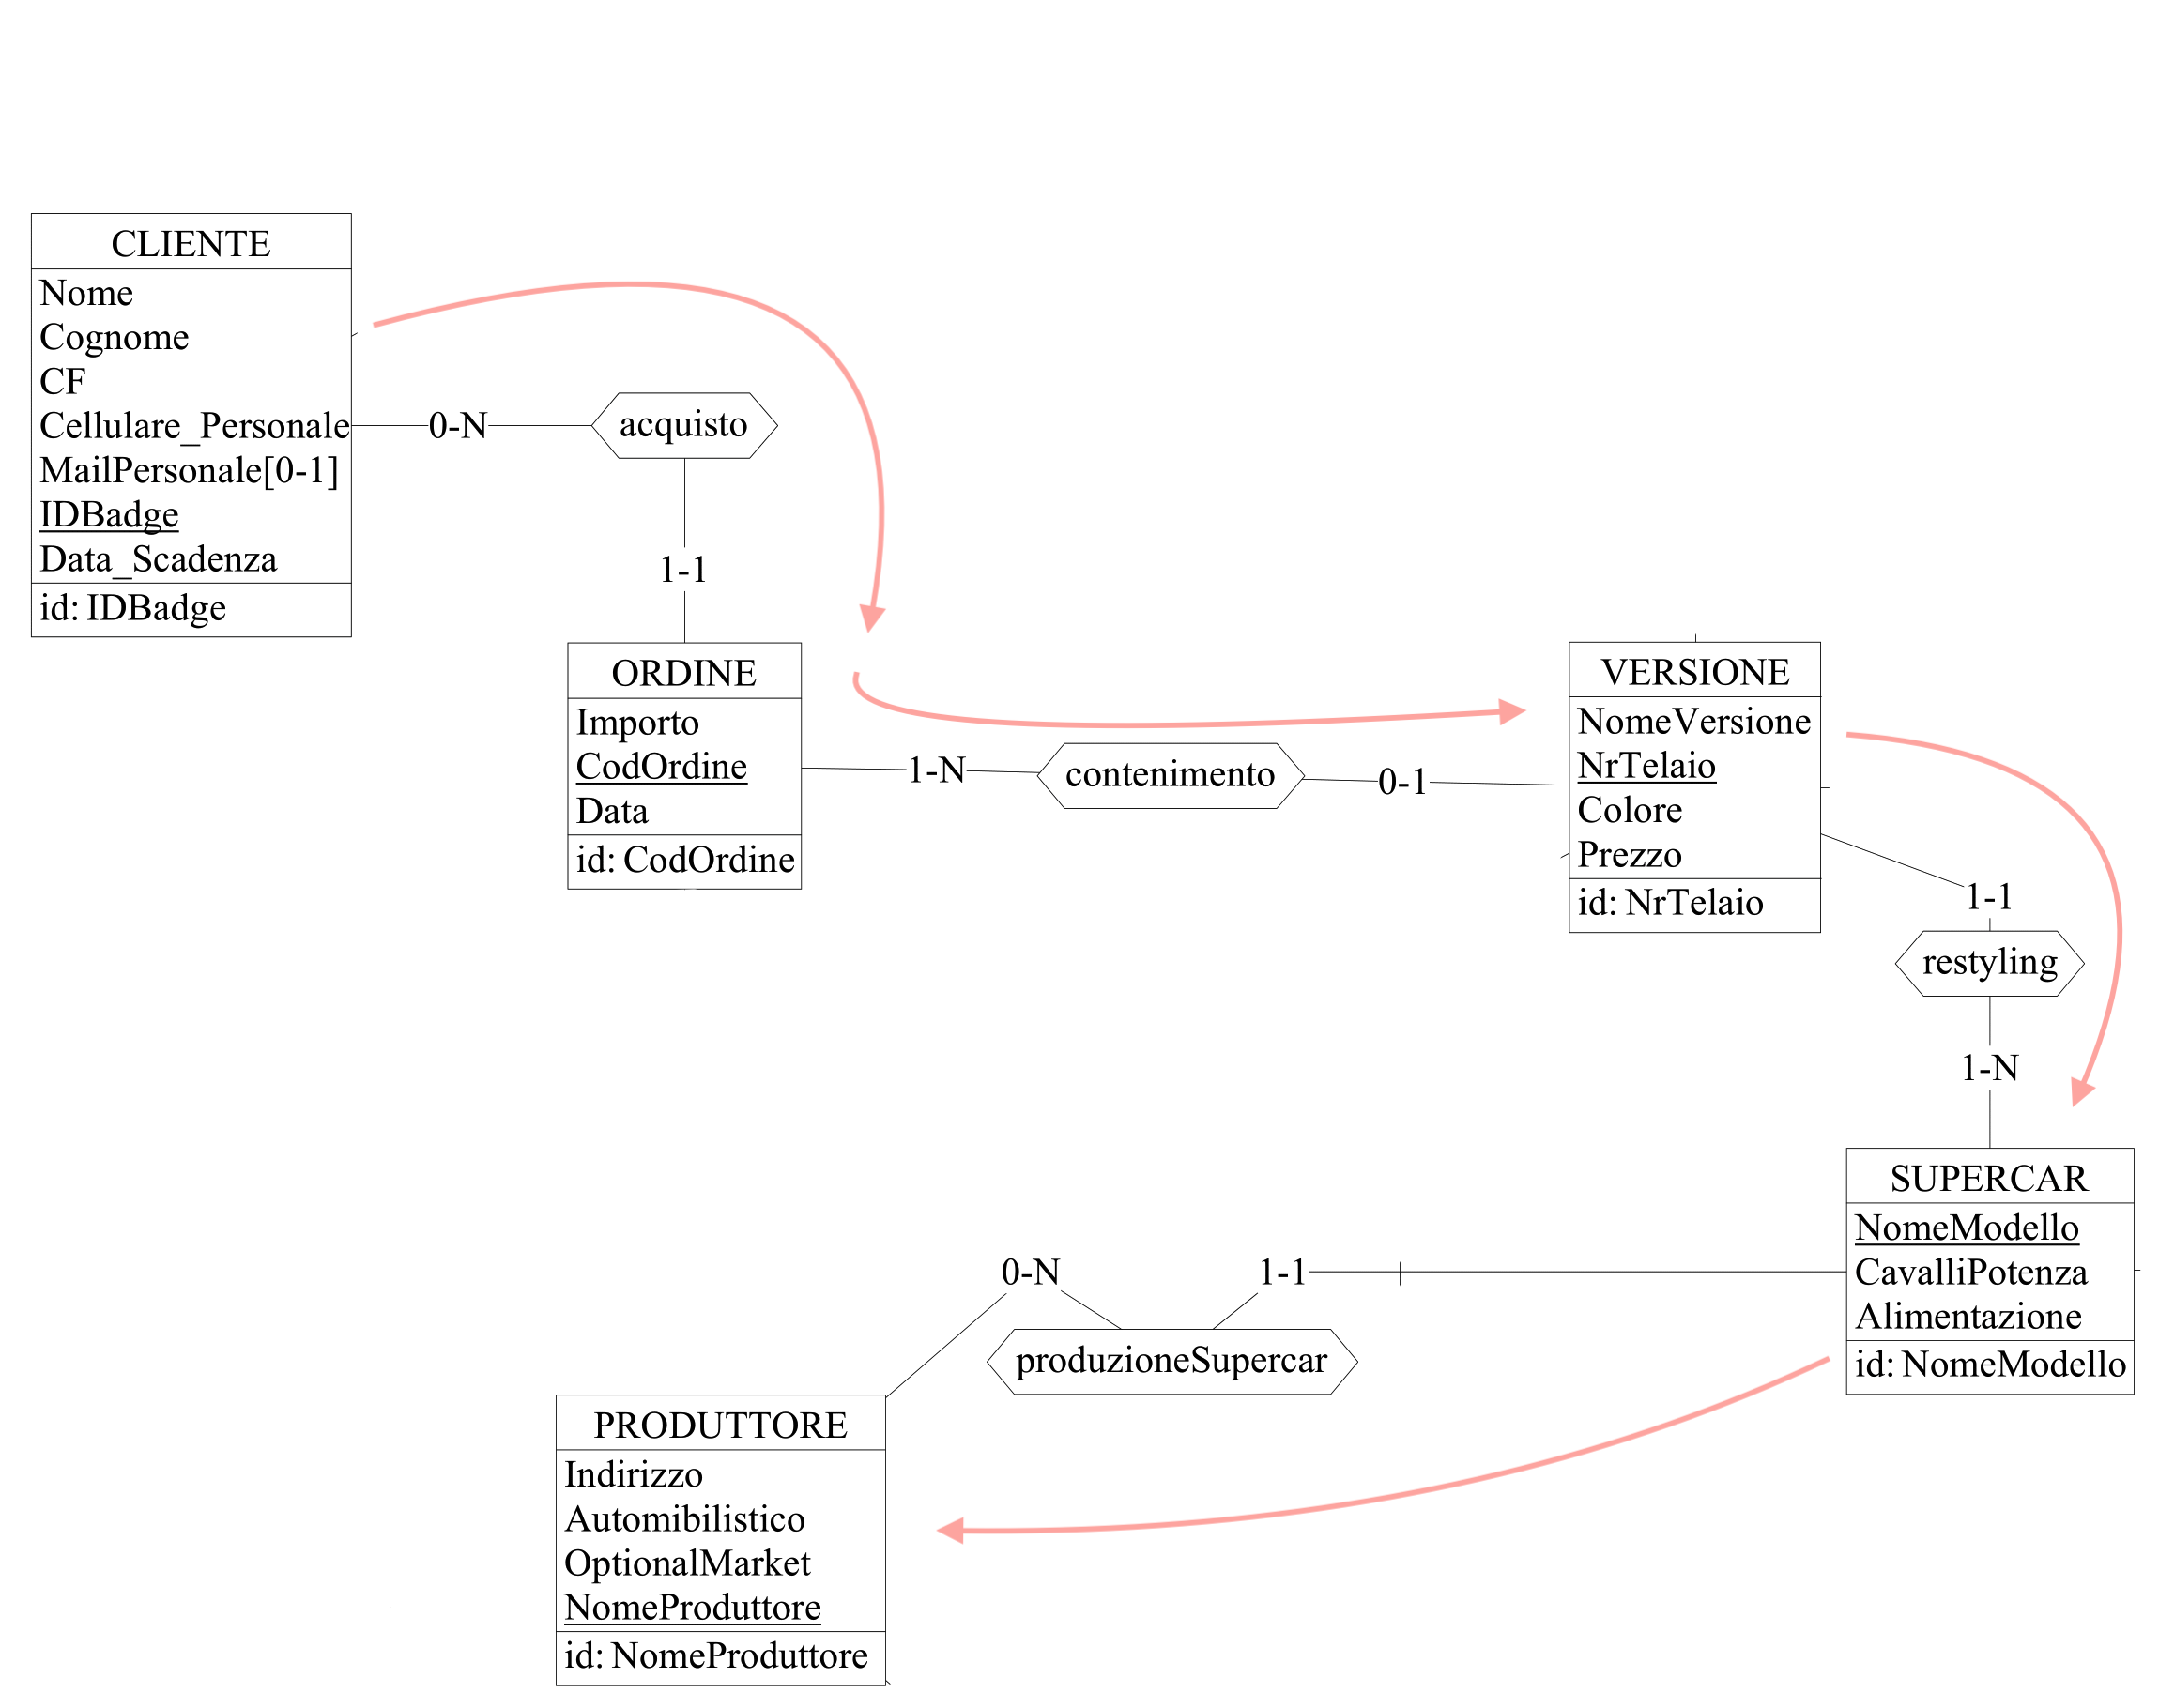
\includegraphics[scale=0.50]{images/navigationSchemes/ordiniCliente.png}
\end{center}

\subsubsection{Visualizza gli optional di una certa azienda} 

Data una certa azienda vado a leggere tutti gli optional che produce. Mediamente
saranno 10'000 Optional / 300 Aziende produttrici di optional = 33 .

\begin{table}[H]
    \centering
    \rowcolors{2}{red!5!}{white}
    \begin{tabular}{ c c c c } 
        \rowcolor{red!20!}
        \textbf{Concetto} & \textbf{Costrutto} & \textbf{Accessi} &
        \textbf{Tipo}\\ 
        PRODUTTORE OPTIONAL & E & 1 & L \\ 
        produzioneOptional & A & 33 & L \\
        OPTIONAL & E & 33 & L \\ 
    \end{tabular}\\
    \( 67L \rightarrow 20\) al mese = \( 34 \times 20 = 1340 \) al mese
\end{table}

\subsubsection{Inserimento di un nuovo ordine} 

\begin{table}[H]
    \centering
    \rowcolors{2}{red!5!}{white}
    \begin{tabular}{ c c c c } 
        \rowcolor{red!20!}
        \textbf{Concetto} & \textbf{Costrutto} & \textbf{Accessi} &
        \textbf{Tipo}\\ 
        DIPENDETE & E & 1 & L \\
        vendita & A & 1 & S \\
        ORDINE & E & 1 & S \\ 
        acquisto & A & 1 & S \\
        CLIENTE & E & 1 & L \\  
        contenimento & A & 1 & S \\
        VERSIONE & E & 2 & L \\
        restyling & A & 2 & L \\
        SUPERCAR & E & 2 & L \\ 
        equipaggiamento & A & 22 & S \\
        OPTIONAL & A & 22 & S \\
    \end{tabular}\\
    \( 48S + 52L \rightarrow \) 66 al mese = \( 48S \times 2 \times 66 + 52L \times
    66 = 9.768\) al mese
\end{table}

\begin{center}
    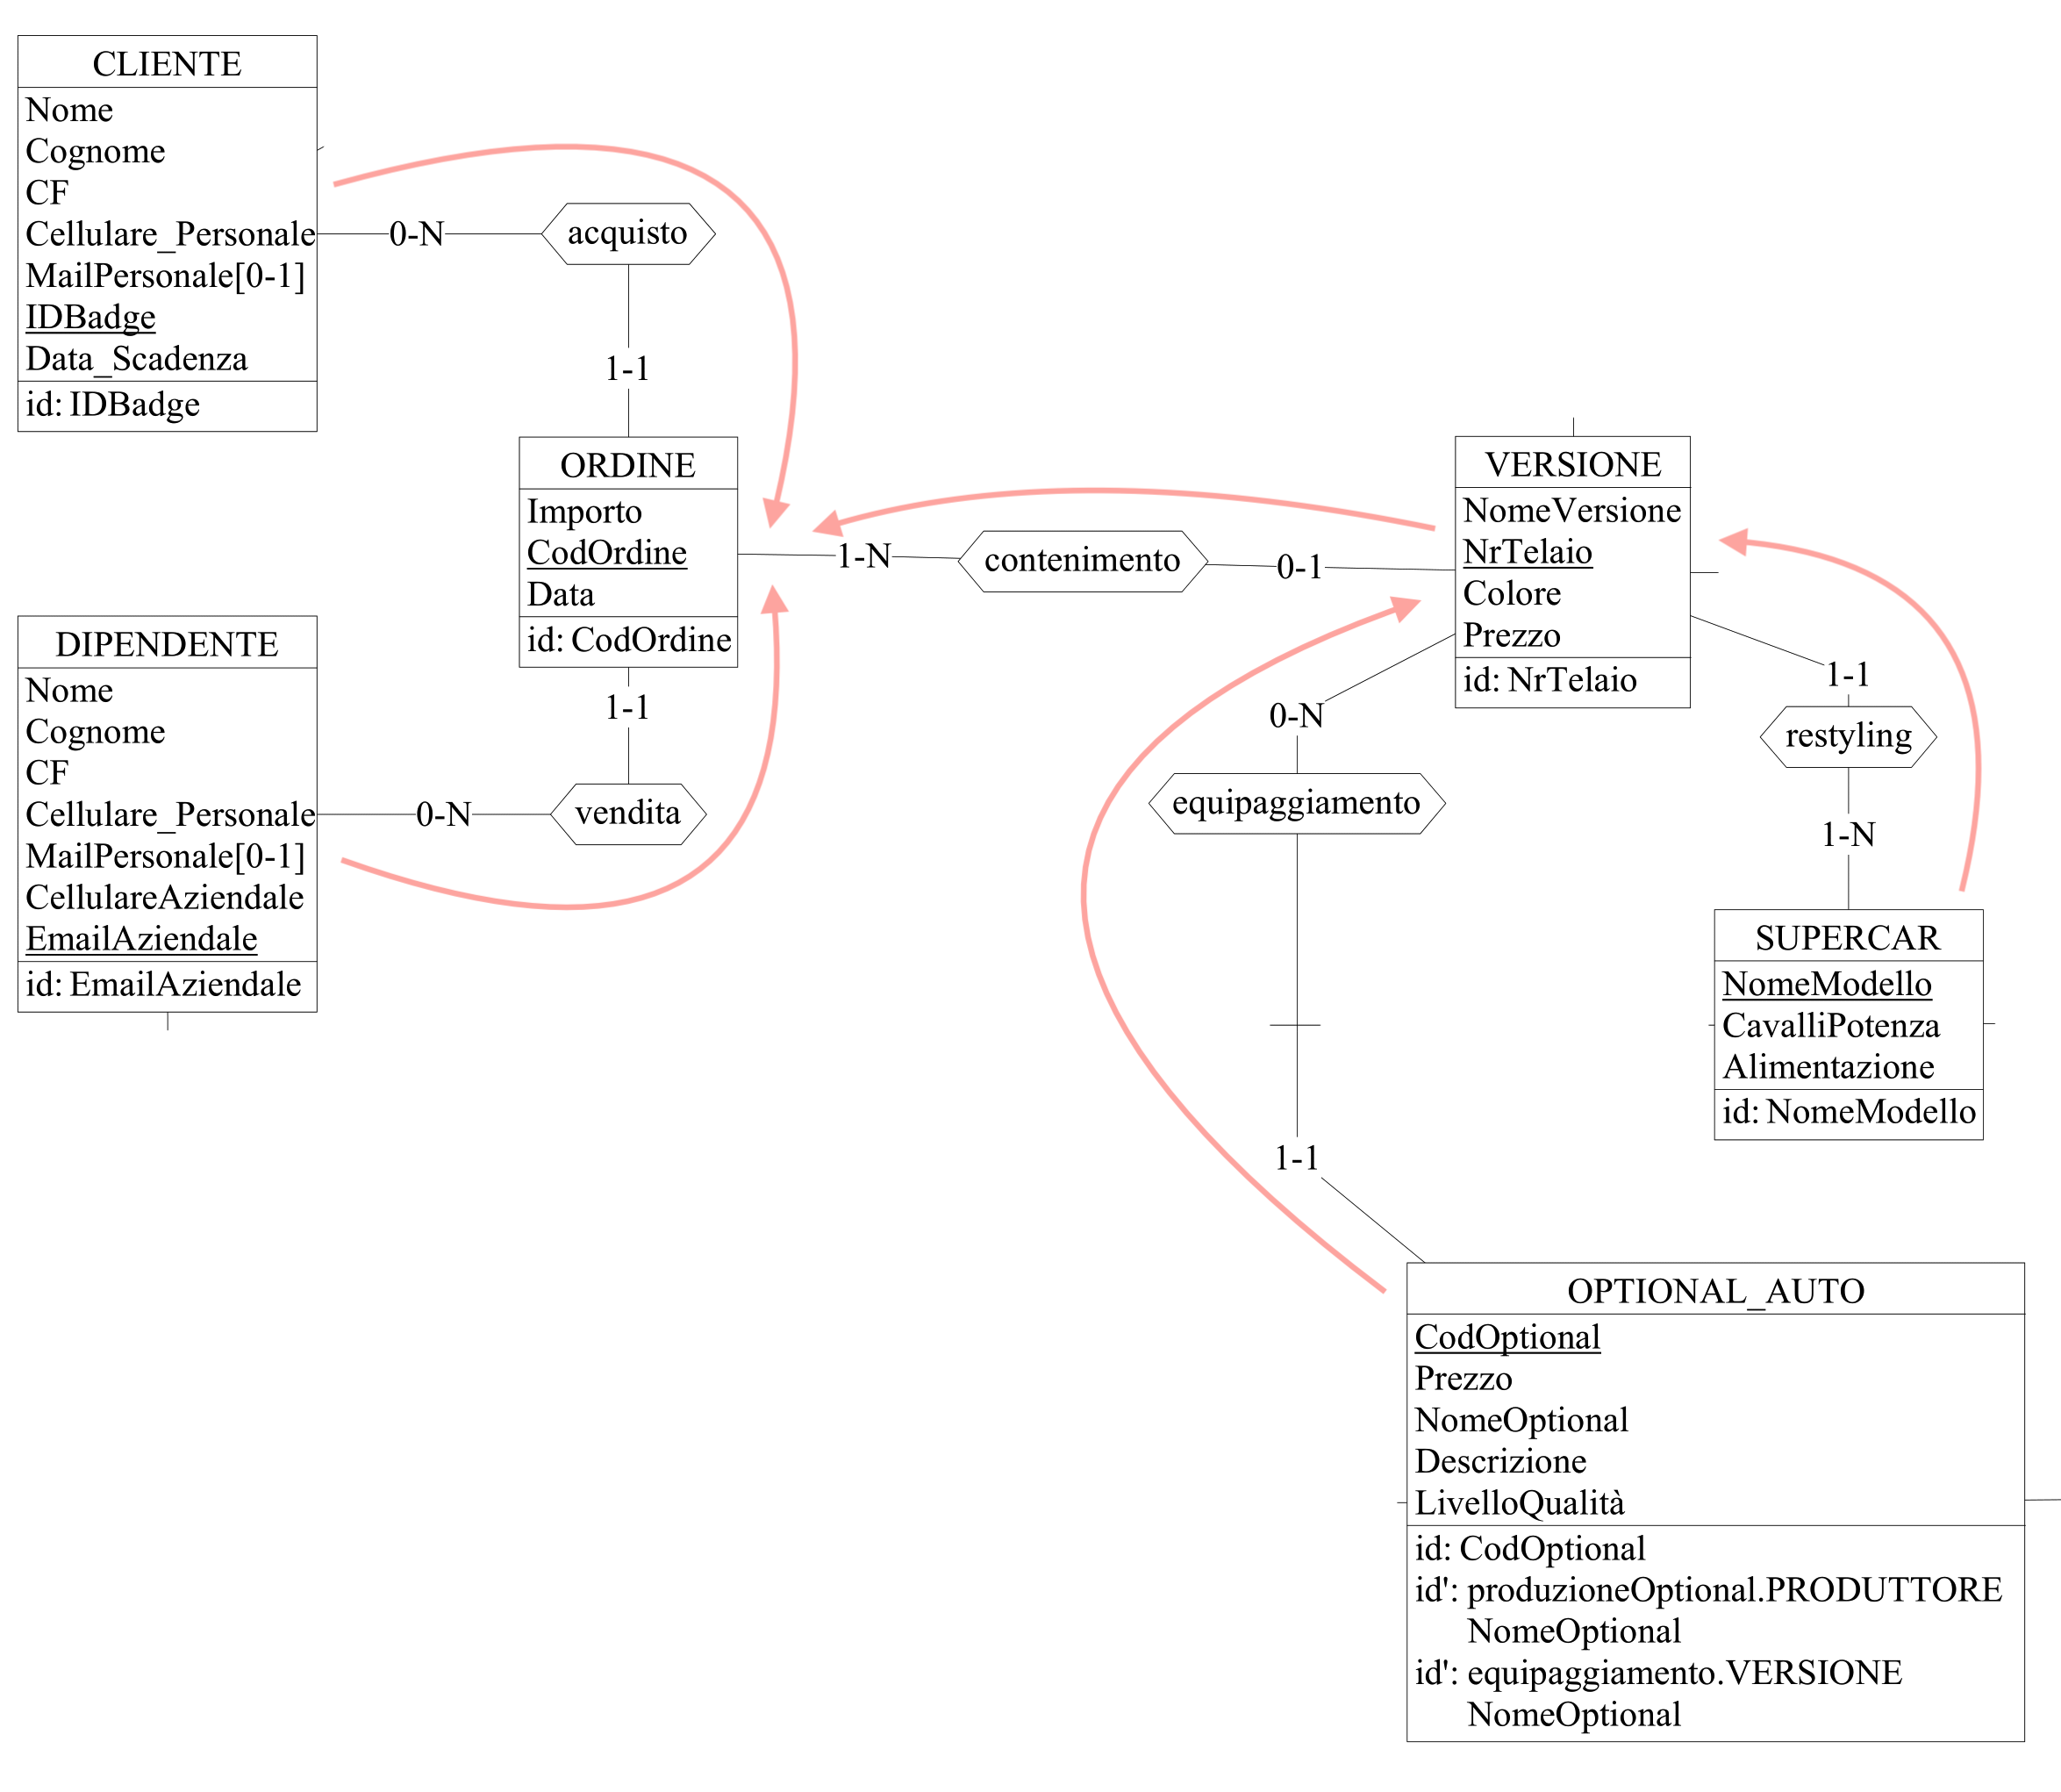
\includegraphics[width=\linewidth]{images/navigationSchemes/creaOrdine.png}
\end{center}

\subsubsection{Aggiungere un contratto di conto vendita}

La valutazione della seguente operazione è stata fatta considerando un nuovo
veicolo non presente nel database ne tra le vetture vendute ne tra quelle
invendute.

\begin{table}[H]
    \centering
    \rowcolors{2}{red!5!}{white}
    \begin{tabular}{ c c c c } 
        \rowcolor{red!20!}
        \textbf{Concetto} & \textbf{Costrutto} & \textbf{Accessi} &
        \textbf{Tipo}\\ 
        CONTO VENDITA & E & 1 & S \\ 
        piazzamento & A & 1 & S \\
        CLIENTE & E & 1 & L \\ 
        relazione & A & 1 & S \\
        VERSIONE & E & 1 & S \\ 
        restyling & A & 1 & S \\
        SUPERCAR & E & 1 & S \\ 
    \end{tabular}\\
    \(6S + 1L \rightarrow \) 1.6 al mese = \( 6S \times 2 \times 1.6 + 1L \times
    1.6 = 20.8 \) al mese  
\end{table}

\subsubsection{Visualizza i dipendenti che in un certo mese hanno ottenuto il
bonus} 

\begin{table}[H]
    \centering
    \rowcolors{2}{red!5!}{white}
    \begin{tabular}{ c c c c } 
        \rowcolor{red!20!}
        \textbf{Concetto} & \textbf{Costrutto} & \textbf{Accessi} &
        \textbf{Tipo}\\ 
        DIPENDENTE & E & 30 & L \\ 
        pagamento & A & 30 & L \\
        STIPENDIO & E & 30 & L \\ 
    \end{tabular}\\
    \( 90L \rightarrow 12 \) all'anno = \( 1080 \) all'anno
\end{table}

\begin{center}
    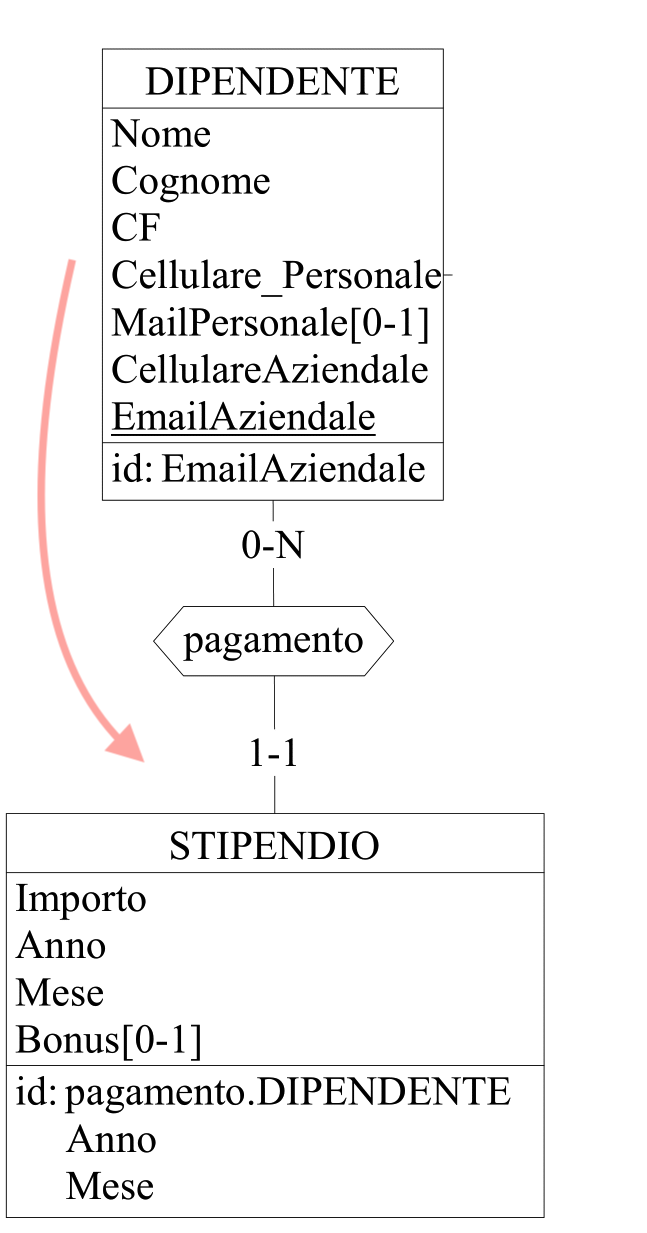
\includegraphics[scale=0.53]{images/navigationSchemes/bonusDipendente.png}
\end{center}

\subsubsection{Visualizza Top 10 supercar più veloci di un segmento e calcola la
media dei cavalli potenza}

Dato un certo segmento vado a ordinare le supercar appartenenti prendendo come
parametro i Cavalli Potenza. In media abbiamo 900 supercar / 10 segmenti = 90
supercar per segmento.

\begin{table}[H]
    \centering
    \rowcolors{2}{red!5!}{white}
    \begin{tabular}{c c c c }
        \rowcolor{red!20!}
        \textbf{Concetto} & \textbf{Costrutto} & \textbf{Accessi} &
        \textbf{Tipo}\\
        SEGMENTO & E & 1 & L \\
        categorizzazione & A & 90 & L \\
        SUPERCAR & E & 90 & L \\
    \end{tabular}\\
    \( 181L  \rightarrow  3 \) al mese = \( 543 \) al mese
\end{table}

\begin{center}
    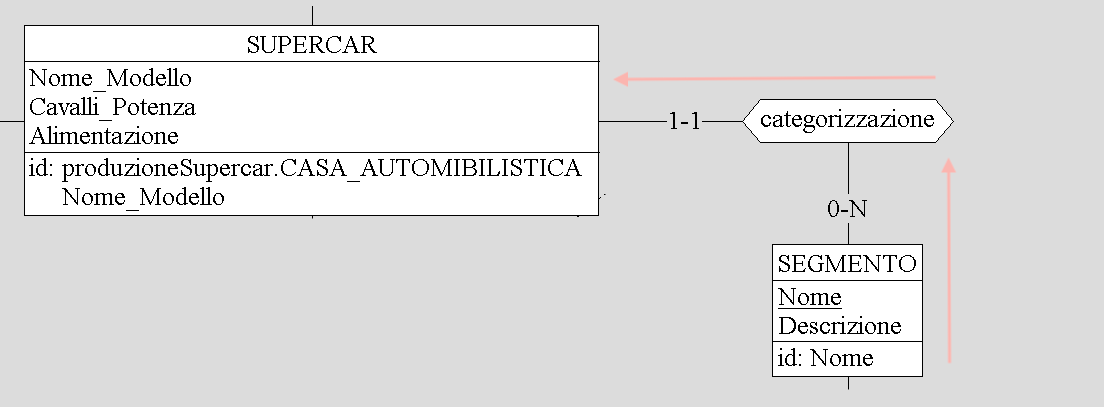
\includegraphics[width=\linewidth]{images/navigationSchemes/supercarSegmento.png}
\end{center}

\subsubsection{Inserisci una nuova versione di una supercar} 

\begin{table}[H]
    \centering
    \rowcolors{2}{red!5!}{white}
    \begin{tabular}{c c c c}
        \rowcolor{red!20!}
        \textbf{Concetto} & \textbf{Costrutto} & \textbf{Accessi} &
        \textbf{Tipo}\\
        SUPERCAR & E & 1 & L \\
        restyling & A & 1 & S \\
        VERSIONE & E & 1 & S \\
    \end{tabular}\\
    \( 1L + 2S \rightarrow 75 \) al mese = \( 1L \times 75 + 2S \times 2 \times
    75 = 375 \) al mese
\end{table}

\subsubsection{Visualizzare l'importo totale di un ordine} 

Mediamente una vettura equipaggia 10'000 optional / 900 versioni = 11 optional per vettura.

\begin{table}[H]
    \centering
    \rowcolors{2}{red!5!}{white}
    \begin{tabular}{c c c c}
        \rowcolor{red!20!}
        \textbf{Concetto} & \textbf{Costrutto} & \textbf{Accessi} &
        \textbf{Tipo}\\
        ORDINE & E & 1 & L \\
        contenimento & A & 2 & L \\
        VERSIONE & E & 2 & L \\
        restyling & A & 2 & L \\
        SUPERCAR & E & 2 & L \\
        equipaggiamento & A & 11 & L \\
        OPTIONAL & E & 11 & L \\
    \end{tabular}\\
    \( 31L \rightarrow 100 \) al mese = \( 3100 \) al mese
\end{table}

\begin{center}
    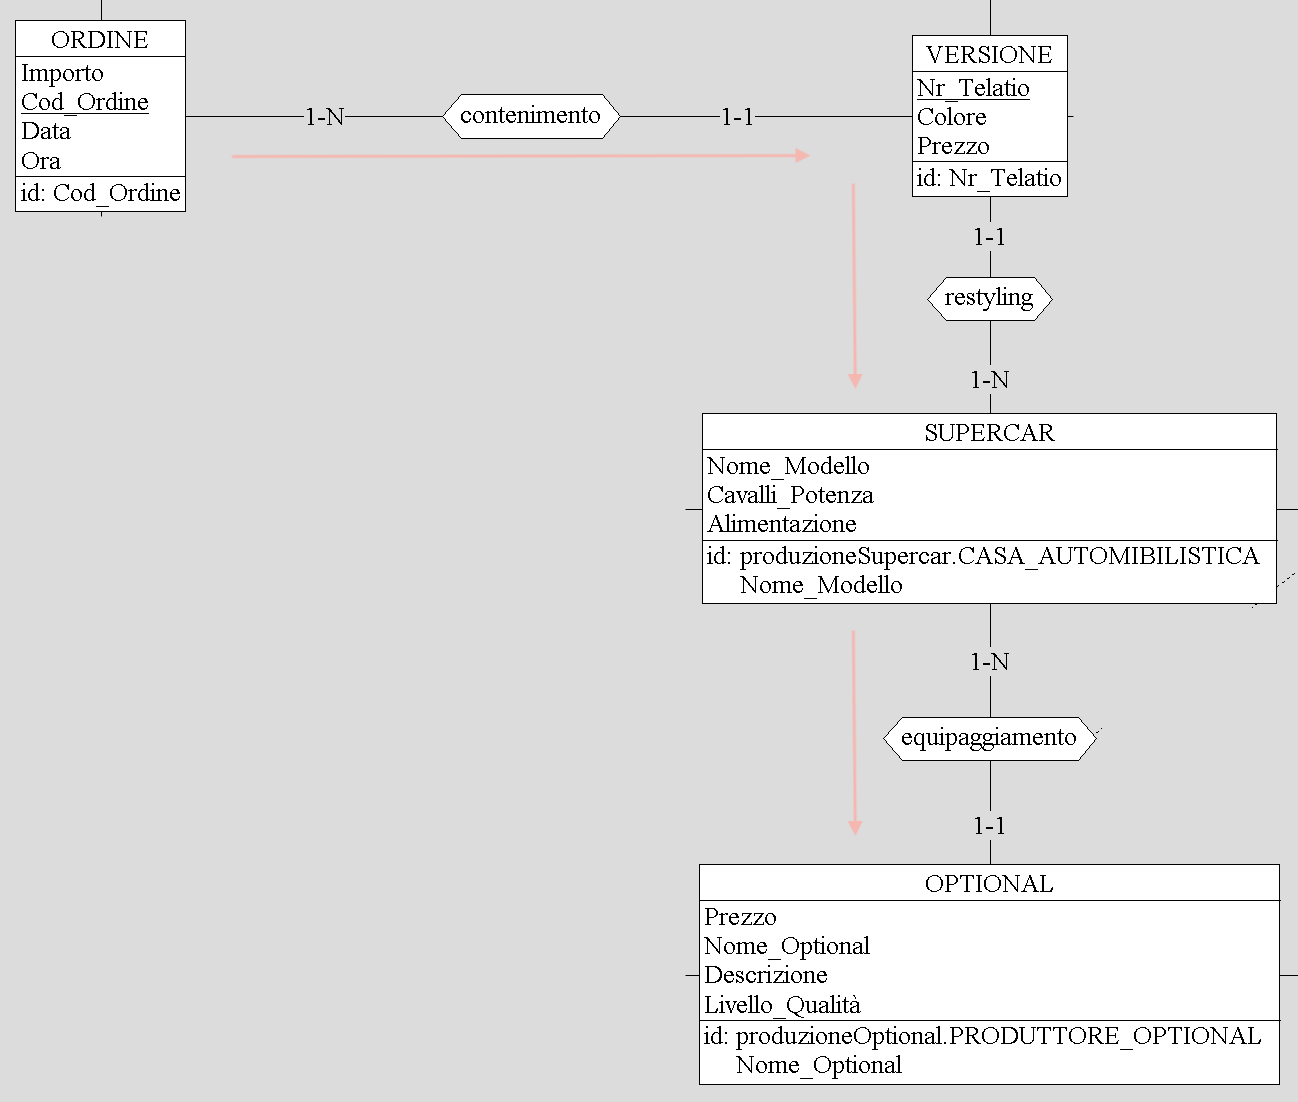
\includegraphics[width=\linewidth]{images/navigationSchemes/calcolaOrdine.png}
\end{center}

\subsubsection{Calcola la spesa annuale in risorse umane della concessionaria}

Si ipotizzano 14 mensilità e che non ci siano state nuove assunzioni o licenziamenti.

\begin{table}[H]
    \centering
    \rowcolors{2}{red!5!}{white}
    \begin{tabular}{c c c c}
        \rowcolor{red!20!}
        \textbf{Concetto} & \textbf{Costrutto} & \textbf{Accessi} &
        \textbf{Tipo}\\
        DIPENDENTE & E & 30 & L \\
        pagamento & A & 420 & L \\
        STIPENDIO & E & 420 & L \\
    \end{tabular}\\
    \( 870L \rightarrow 5 \) all'anno = \( 4350 \) all'anno
\end{table}

\subsection{Raffinamento dello schema (eliminazione di identificatori esterni,
attributi composti e gerarchie, scelta delle chiavi)}

\subsubsection{Attributi Composti}
\begin{itemize}
    \item Gli attributi composti sono stati ristrutturati come semplici
    attributi appartenenti alla rispettiva Entità. Questo processo è stato
    attuato sia sulla entità MANUTENZIONE che in quella PRODUTTORE.
\end{itemize}

\subsubsection{Eliminazione delle Gerarchie}

\begin{itemize}
    \item Nel caso di CLIENTE e DIPENDENTE, entrambi un estensione di persona,
    ho attuato un collasso verso il basso in quanto si tratta di copertura
    Totale ed Esclusiva.
    \item Nel caso di CASE AUTOMOBILISTICA e di PRODUTTORE OPTIONAL, invece,
    essendo una copertura sovrapposta ho unito le 2 entità nella unica entità
    PRODUTTORE in quanto la logica viene mantenuta anche differenziando le
    entità con attributi booleani utili a definire la differenza da un produttore e
    l'altro.
\end{itemize}

\subsubsection{Scelta delle Chiavi}

Di seguito riporto una tabella che riassume le chiavi scelte per ogni entità.

\begin{center}
    \begin{table}[htbp]
        \centering
        \small
        \rowcolors{2}{red!5!}{white}
        \begin{tabularx}{\textwidth}{l l}
            \rowcolor{red!20!}
            \textbf{Concetto} & \textbf{Chaive Primaria}\\
            CLIENTE & IDBadge \\
            DIPENDENTE & EmailAziendale \\
            ORDINE & CodOrdine \\
            CONTOVENDITA & CodContratto \\
            VERSIONE & NrTelaio \\
            SUPERCAR & NomeModello \\
            SEGMENTO & NomeSegemento \\
            PRODUTTORE & NomeProduttore \\
            STIPENDIO & DIPENDENTE(EmailAziendale), Anno, Mese \\
            MANUTENZIONE & VERSIONE(NrTelaio), Anno \\
            OPTIONAL-AUTO & CodOptional \\
            SUPERCAR & PRODUTTORE(NomeProduttore), NomeModello \\
        \end{tabularx}
    \end{table}    
\end{center}

\newpage

\subsection{Analisi delle ridondanze}

La presenza del attributo \textit{Importo} al intero di Ordine comporta una
ridondanza in quanto è un valore calcolabile anche mediante somme dei prezzi dei
prodotti presenti nel ordine. Si vuole valutare la presenza di questo attributo.\\

L'operazione ``Visualizzare l'importo totale di un ordine" è una delle più
frequenti ed è utile per misurare l'efficienza di questo attributo.

\begin{table}[H]
    \centering
    \rowcolors{2}{red!5!}{white}
    \begin{tabular}{c c c c}
        \rowcolor{red!20!}
        \textbf{Concetto} & \textbf{Costrutto} & \textbf{Accessi} &
        \textbf{Tipo}\\
        ORDINE & E & 1 & L \\
    \end{tabular}\\
    \( 1L \rightarrow 100 \) al mese = \( 100 \) al mese
\end{table}

Inserire questa ridondanza appesantisce il database ma velocizza le operazioni e
risulterebbe utile anche per ulteriori operazioni statistiche. 
Si decide quindi di mantere l'attributo \textit{Importo} nella entità ORDINE.

\newpage

\subsection{Schema Logico}

\begin{center}
    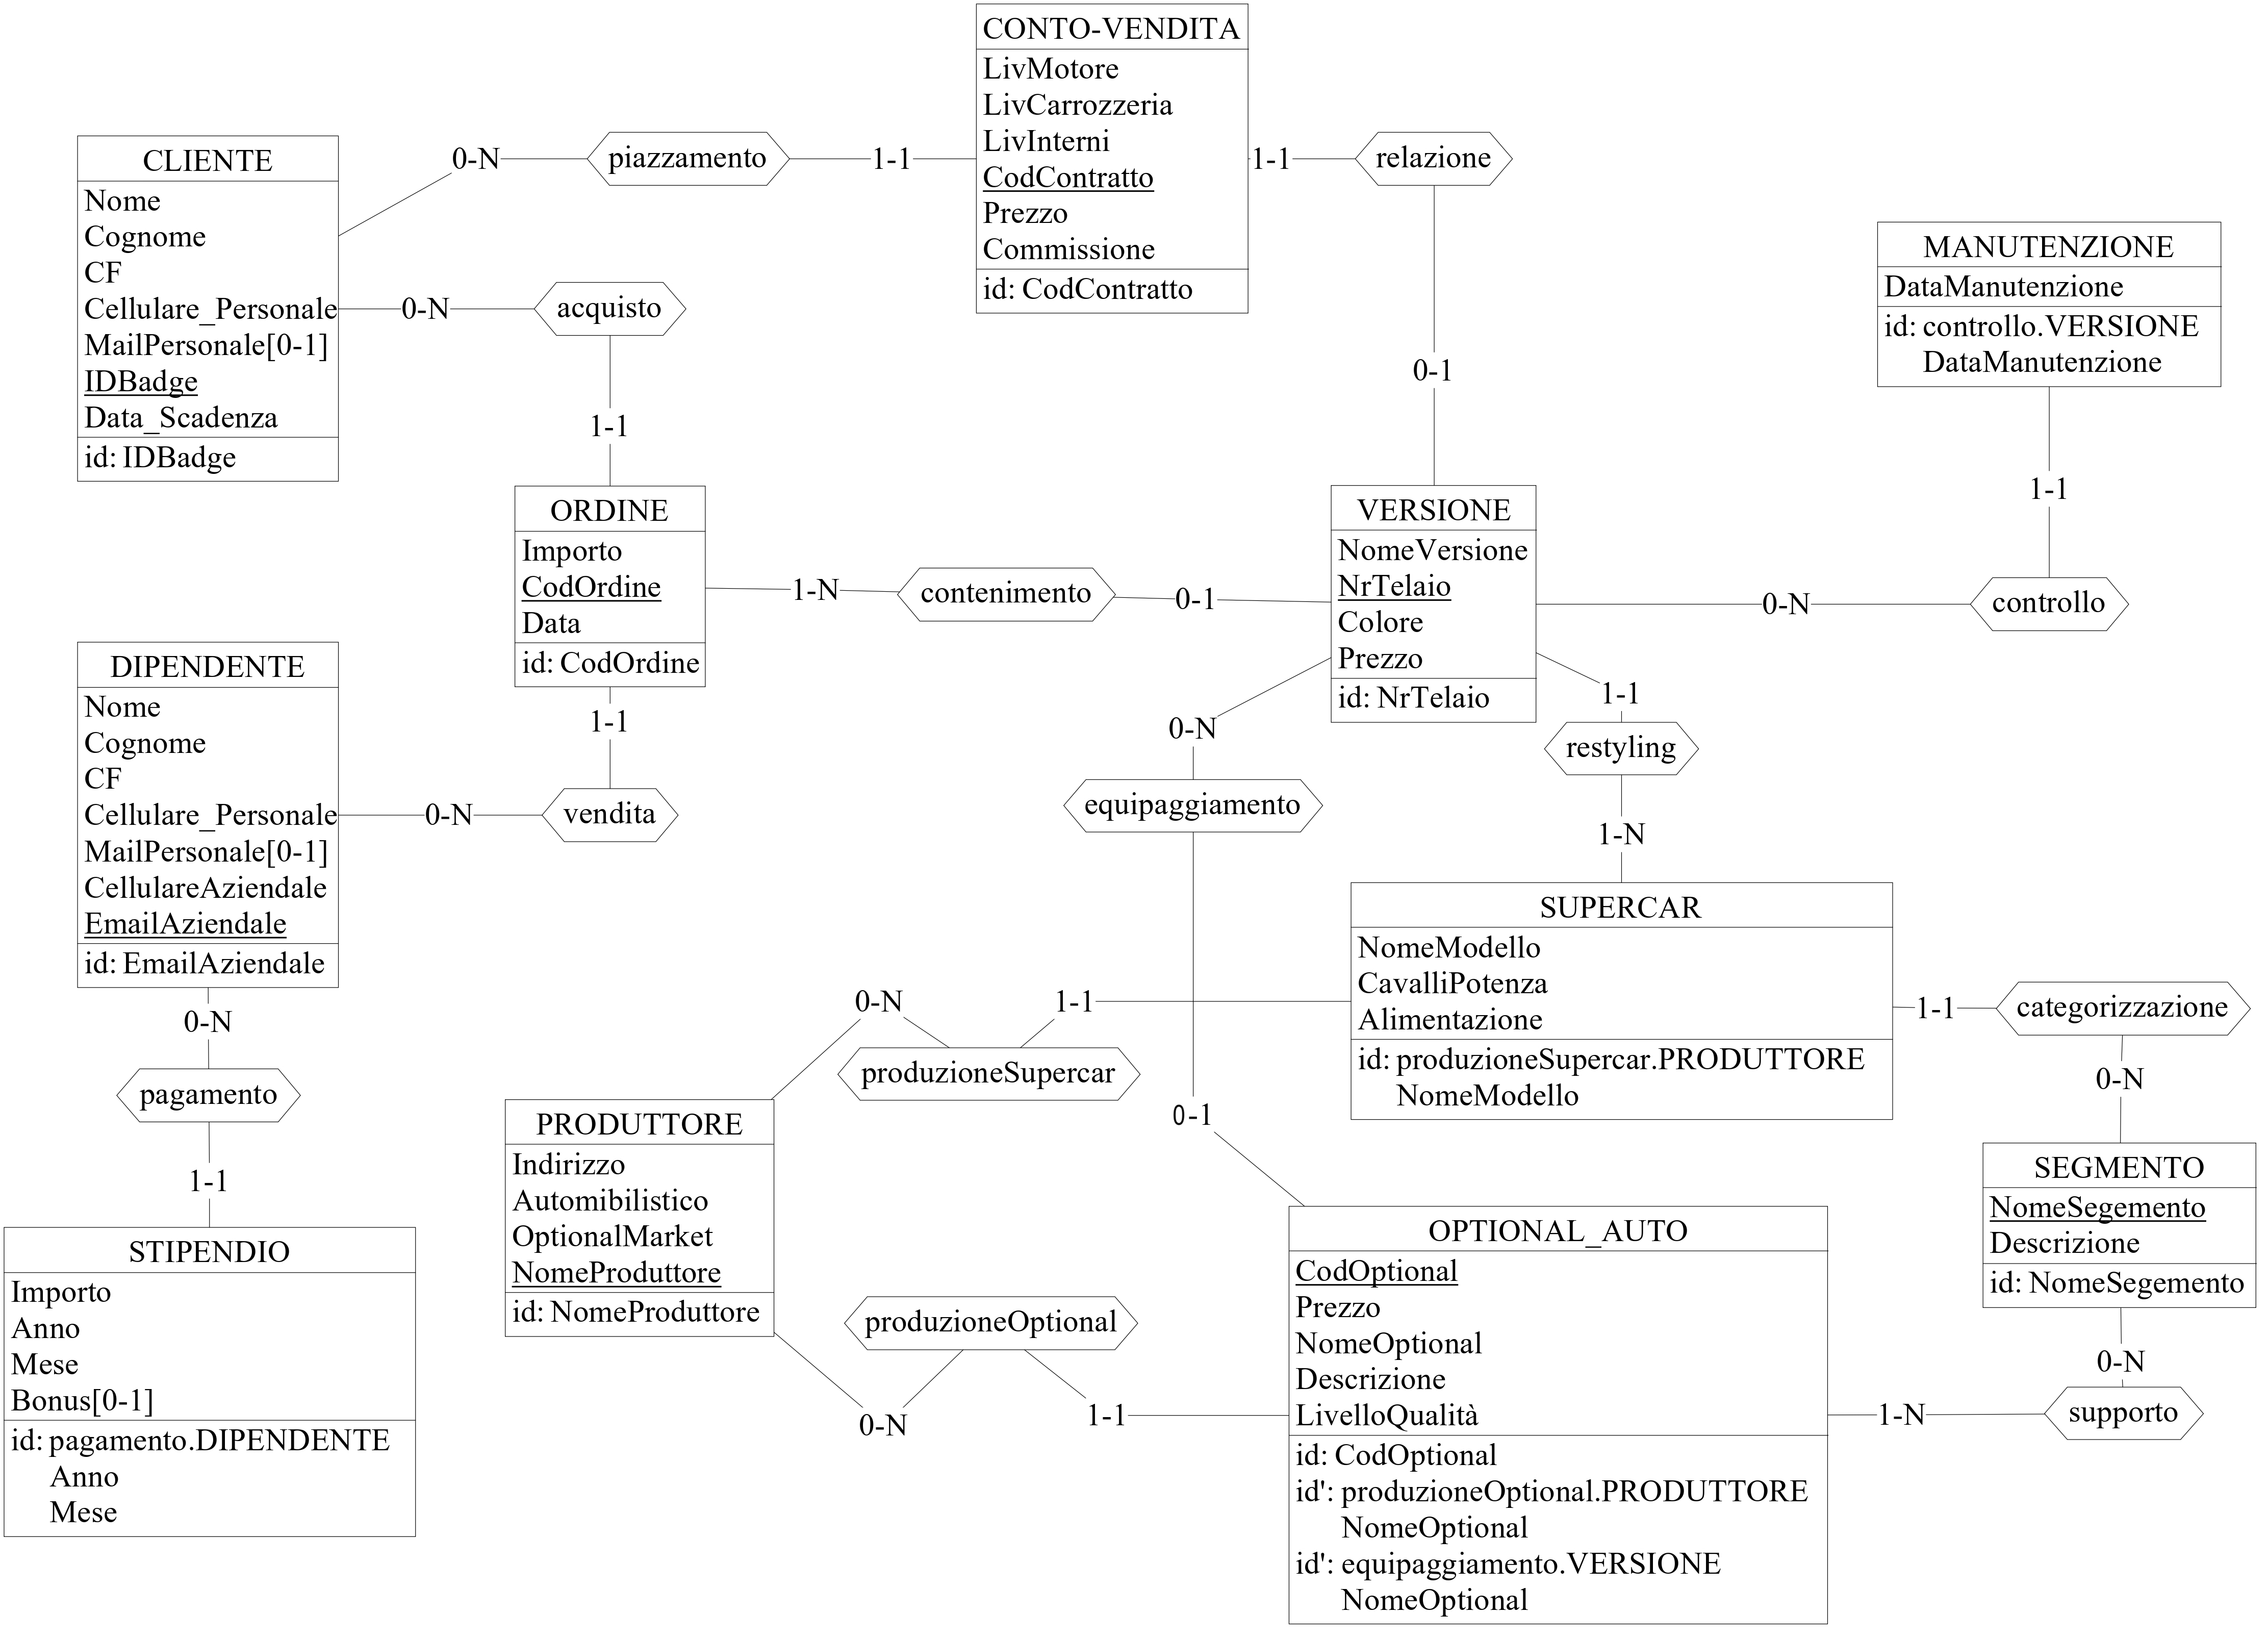
\includegraphics[height=\linewidth, angle=90]{images/fullSchemes/logico.jpeg}
\end{center}

\newpage

\subsection{Traduzione di entità e associazioni in relazioni}

\small

\begin{flushleft}
CLIENTI(\underline{IDBadge}, DataScadenza, Nome, Cognome, CF,
    CellularePersonale, MailPersonale*)\\
UNIQUE(CF, CellularePersonale, MailPersonale)
\end{flushleft}
    

\begin{flushleft}
DIPENDENTI(\underline{EmailAziendale}, Nome, Cognome, CF, CellularePersonale,
MailPersonale*, CellulareAziendale)\\
UNIQUE(CellularePersonale, MailPersonale, CellulareAziendale, CF)
\end{flushleft}

\begin{flushleft}
STIPENDI(\underline{EmailAziendale}, Importo, Anno, Mese, Bonus*)\\
FK EmailAziendale REFERENCES DIPENDENTI
\end{flushleft}

\begin{flushleft}
ORDINI(\underline{CodOrdine}, Data, Ora, Importo, EmailAziendale, IDBadge)\\
FK EmailAziendale REFERENCES DIPENDENTI\\
FK IDBadge REFERENCES CLIENTI
\end{flushleft}

\begin{flushleft}
CONTOVENDITA(\underline{CodContratto}, Prezzo, Commissione, LivMotore,
LivCarrozzeria, LivInterni, IDBadge, NrTelaio)\\
FK IDBadge REFERENCES CLIENTI\\
FK NrTelaio REFERENCES VERSIONI
\end{flushleft}

\begin{flushleft}
VERSIONI(\underline{NrTelaio}, NomeVersione, Prezzo, Colore, CodContratto*, NomeModello, CodOrdine*)\\
FK NomeModello REFERENCES SUPERCAR
FK CodOrdine REFERENCES ORDINI
FK CodContratto REFERENCES CONTOVENDITE
\end{flushleft}

\begin{flushleft}
MANUTENZIONE(\underline{DataManutenzione}, \underline{NrTelaio})\\
FK NrTelaio REFERENCES VERSIONI
\end{flushleft}

\begin{flushleft}
SUPERCAR(\underline{NomeModello}, \underline{NomeProduttore}, CavalliPotenza, NomeSegmento)\\
FK NomeProduttore REFERENCES PRODUTTORI\\
FK NomeSegmento REFERENCES SEGMENTI
\end{flushleft}

\begin{flushleft}
SEGMENTI(\underline{NomeSegmento}, Descrizione)
\end{flushleft}

\begin{flushleft}
supporto(\underline{NomeSegmento}, \underline{CodOptional})
FK NomeSegmento REFERENCES SEGMENTI
FK CodOptional REFERENCES OPTIONAL-AUTO
\end{flushleft}

\begin{flushleft}
PRODUTTORI(\underline{NomeProduttore}, Automobilistico, OptionalMarket, Indirizzo)
\end{flushleft}

\begin{flushleft}
OPTIONAL-AUTO(\underline{CodOptional}, \underline{NomeProduttore}, \underline{NomeOptional}, Prezzo, Descrizione, LivelloQualità, NrTelaio*)\\
FK NomeProduttore REFERENCES PRODUTTORI
FK NrTelaio REFERENCES VERSIONI
\end{flushleft}

\normalsize

\newpage 

\subsection{Schema relazionale finale}

\begin{center}
    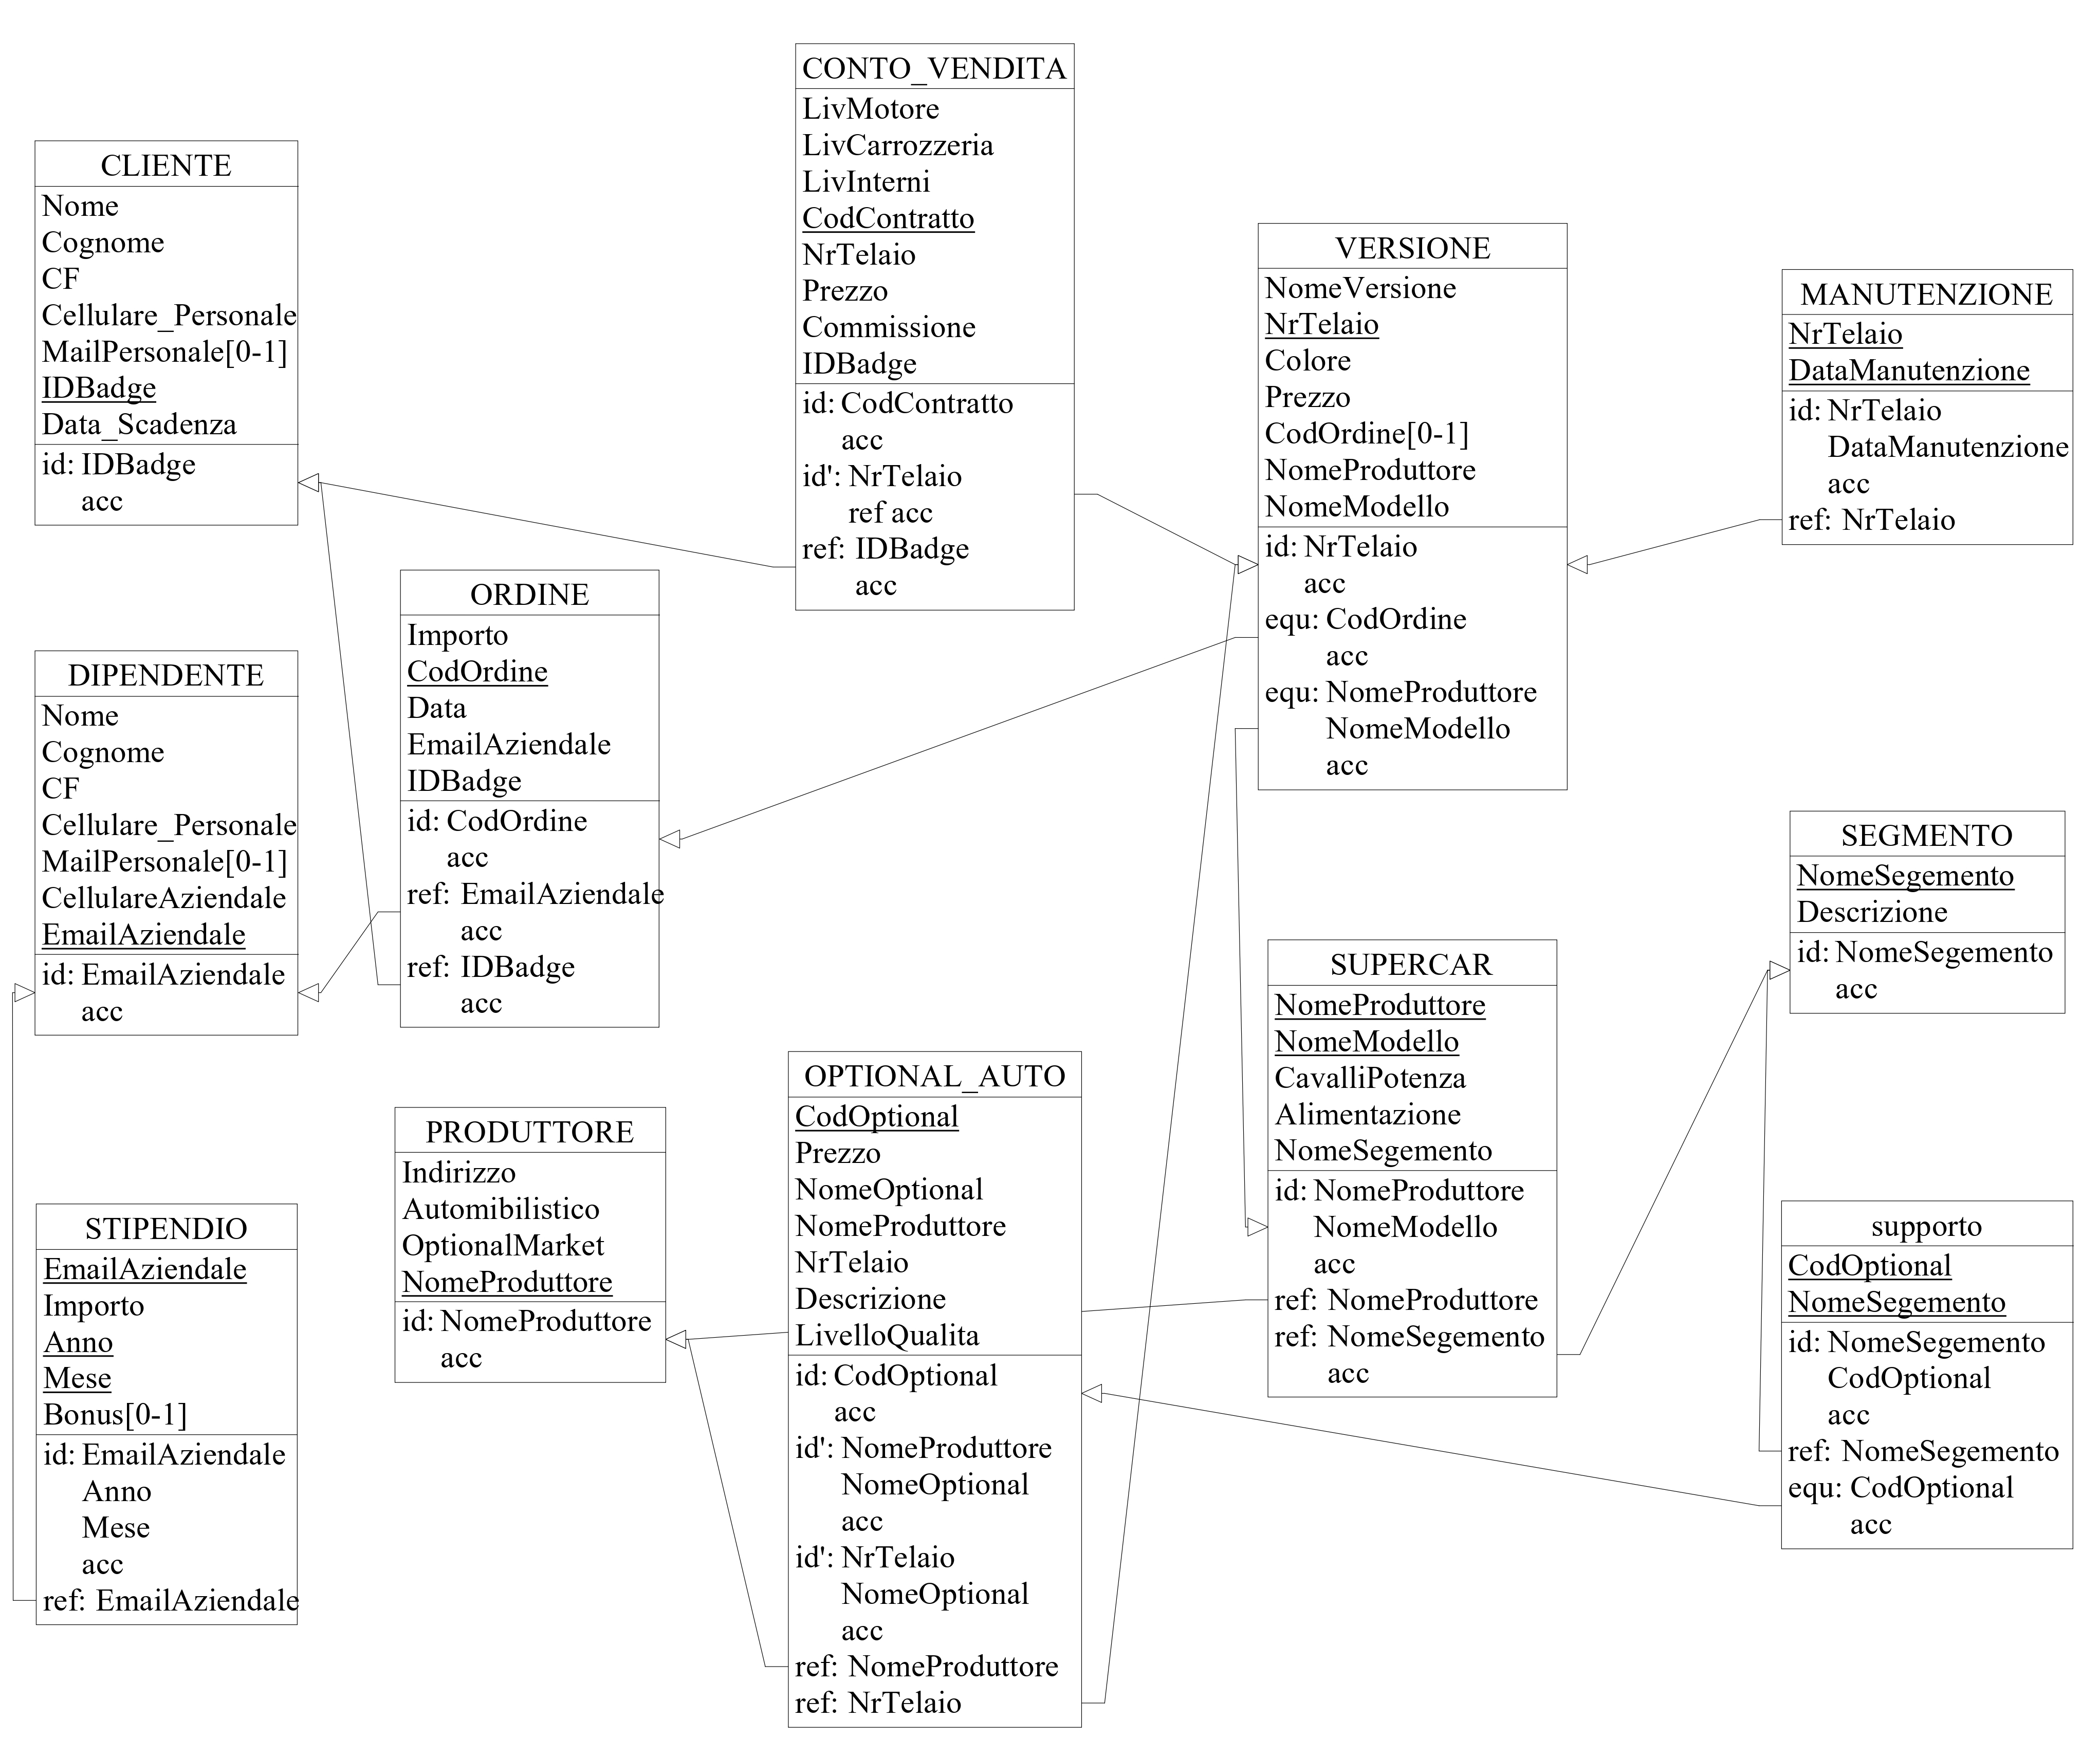
\includegraphics[height=\linewidth, angle=90]{images/fullSchemes/relazionale.jpeg}
\end{center}

\newpage

\lstset{style=sqlStyle}

\subsection{Traduzione delle operazioni in query SQL}

\subsubsection*{Log In Dipendente}

\begin{lstlisting}
    SELECT * 
    FROM DIPENDENTE 
    WHERE Email_Aziendale = 'Email Dipendente'
\end{lstlisting}
Si verifica che la tabella creata dalla query \\
abbia una riga sola e si effettua il Log In.

\subsubsection*{Inserimento di un nuovo cliente}

\begin{lstlisting}
    INSERT INTO CLIENTE(Nome, Cognome, CF, CellularePersonale, MailPersonale, DataScadenza)
    VALUES (?, ?, ?, ?, ?, date_add(curdate(), INTERVAL 1 YEAR))
\end{lstlisting}

\subsubsection*{Visualizza le vetture acquistate da un cliente in un certo
periodo in ordine crescente di data}

\begin{lstlisting}
    SELECT ORDINE.CodOrdine, PRODUTTORE.NomeProduttore, SUPERCAR.NomeModello, VERSIONE.NomeVersione
    FROM ORDINE, VERSIONE, SUPERCAR, PRODUTTORE
    where ORDINE.IDBadge = ?
    and ORDINE.CodOrdine = VERSIONE.CodOrdine
    and VERSIONE.NomeModello = SUPERCAR.NomeModello
    and SUPERCAR.NomeProduttore = PRODUTTORE.NomeProduttore
    and ORDINE.DataOrdine BETWEEN ? AND ?
    order by ORDINE.DataOrdine DESC;
\end{lstlisting}

\subsubsection*{Visualizza gli optional di una certa azienda}
\begin{lstlisting}
    SELECT NomeOptional, Prezzo, LivelloQualita
    FROM OPTIONAL_AUTO, PRODUTTORE
    WHERE PRODUTTORE.NomeProduttore = ?
    AND OPTIONAL_AUTO.NomeProduttore = PRODUTTORE.NomeProduttore
\end{lstlisting}

\subsubsection*{Inserimento di un nuovo ordine}

Le istruzioni sottostanti sono le principali per l'inserimento di un nuovo
ordine, si rimanda al codice per una visione completa.

\begin{lstlisting}
    INSERT INTO ORDINE(Importo, DataOrdine, EmailAziendale, IDBadge)
    VALUES (0 , current_date(), ?, ?)

    UPDATE VERSIONE
    SET CodOrdine = ?
    WHERE NomeProduttore = ?
    AND NomeModello = ?
    AND NomeVersione = ?

    UPDATE OPTIONAL_AUTO
    SET NrTelaio = ?
    WHERE NomeOptional = ?
\end{lstlisting}

\subsubsection*{Aggiungere un contratto di conto vendita}
\begin{lstlisting}
    INSERT INTO CONTO_VENDITA(LivMotore, LivCarrozzeria, LivInterni, NrTelaio, Prezzo, Commissione, IDBadge)
    VALUES (?, ?, ?, ?, ?, ?, ?);

    UPDATE VERSIONE
    SET VERSIONE.CodOrdine = null, 
            VERSIONE.Prezzo = (SELECT CONTO_VENDITA.Prezzo 
                            FROM CONTO_VENDITA 
                            WHERE CONTO_VENDITA.NrTelaio = VERSIONE.NrTelaio) 
    WHERE VERSIONE.NrTelaio = ?;
\end{lstlisting}

\subsubsection*{Visualizza i dipendenti che in un certo mese hanno ottenuto il
bonus}

\begin{lstlisting}
    SELECT DIPENDENTE.Nome, DIPENDENTE.Cognome, DIPENDENTE.EmailAziendale
    FROM DIPENDENTE, STIPENDIO
    WHERE STIPENDIO.EmailAziendale = DIPENDENTE.EmailAziendale
    AND STIPENDIO.Mese = ?
    AND STIPENDIO.Anno = ?
    AND STIPENDIO.Bonus is not null;
\end{lstlisting}

\subsubsection*{Visualizza Top 10 supercar piu veloci di un segmento}

\begin{lstlisting}
    SELECT PRODUTTORE.NomeProduttore, SUPERCAR.NomeModello, SUPERCAR.CavalliPotenza
    FROM SUPERCAR, PRODUTTORE
    WHERE SUPERCAR.NomeSegemento = ?
    AND SUPERCAR.NomeProduttore = PRODUTTORE.NomeProduttore
    ORDER BY CavalliPotenza DESC
    LIMIT 10;
\end{lstlisting}

\subsubsection*{Inserisci una nuova versione di una supercar}

\begin{lstlisting}
    INSERT INTO VERSIONE(NomeVersione, NrTelaio, Colore, Prezzo, CodOrdine, NomeProduttore, NomeModello)
    VALUES(?, ?, ?, ?, null, ?, ?);
\end{lstlisting}

\subsubsection*{Visualizzare l’importo totale di un ordine}

Questa operazione viene eseguita nel momento di inserimeto di una nuovo ordine.

\begin{lstlisting}
    SELECT Importo
    FROM ORDINE
    WHERE ORDINE.CodOrdine = ?;
\end{lstlisting}

Query di calcolo dell'importo totale di un ordine:

\begin{lstlisting}
    UPDATE ORDINE
    SET ORDINE.Importo = ((SELECT SUM(VERSIONE.Prezzo)
                        FROM VERSIONE 
                        WHERE VERSIONE.CodOrdine = ?) 
                            + (SELECT SUM(OPTIONAL_AUTO.Prezzo)
                                FROM OPTIONAL_AUTO
                                WHERE OPTIONAL_AUTO.NrTelaio 
                                        IN (SELECT VERSIONE.NrTelaio
                                            FROM VERSIONE
                                            WHERE VERSIONE.CodOrdine = ?)))
    WHERE ORDINE.CodOrdine = ?;
\end{lstlisting}

\subsubsection*{Calcola la spesa annuale in risorse umane della concessionaria}

\begin{lstlisting}
    SELECT SUM(STIPENDIO.Importo) + SUM(STIPENDIO.Bonus) AS 'Spesa Annuale'
    FROM STIPENDIO
    WHERE STIPENDIO.Anno = ?;
\end{lstlisting}

\section{Progettazione dell'applicazione}

\subsection{Descrizione dell'architettura dell'applicazione realizzata con
obbligo di inserire alcuni screenshot dell'interfaccia utente}

Si e progettata l'applicazione in C\# con il supporto del package
MySQLConnection Framework. Si e valutato fosse importante una GUI semplice ed
intuitiva che permettesse anche ai nuovi dipendenti di impararne l'utilizzo in
breve tempo.\\
Di seguito gli screenshot di alcune schermate dell'applicazione.

\subsubsection{Pagina di Log In}
Di seguito la schermata di login al sistema. Una query contralla che la mail
inserita sia presente nel database e nel caso positivo permette l'accesso.
\begin{center}
    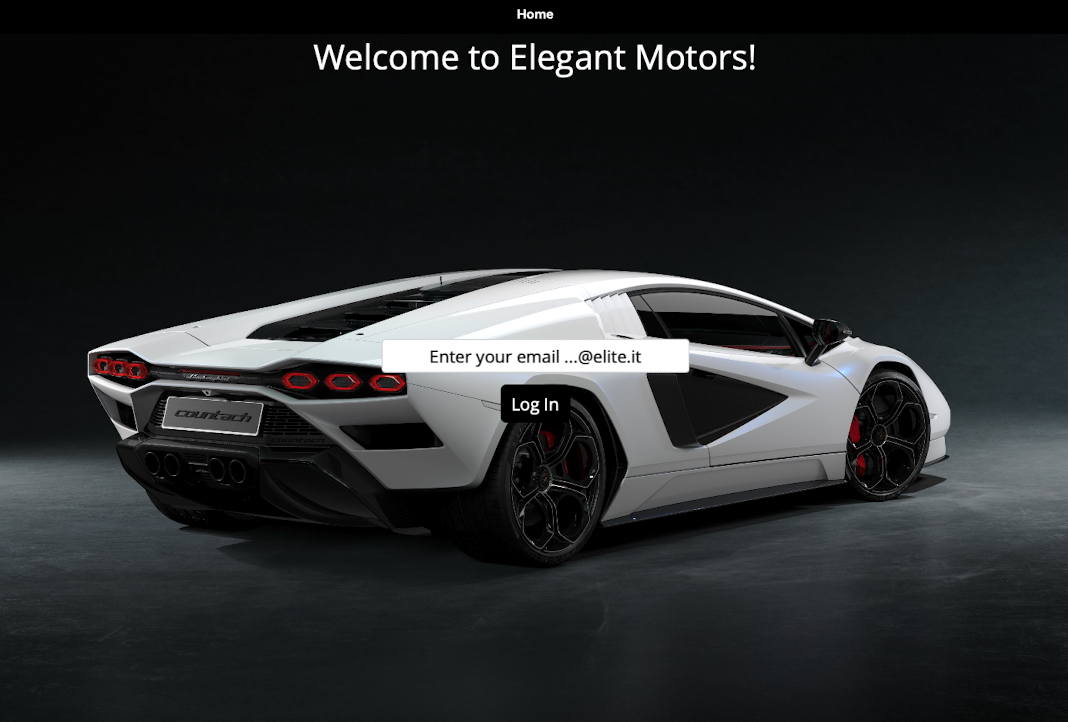
\includegraphics[width=\linewidth]{images/app/logInPage.png}
\end{center}

\subsubsection{Pagine delle Top 10 Supercar più veloci}
Con l'utlizzo di un menu a tendina si riesce a scorrere tra i vari segmenti
e visualizzare le 10 supercar più veloci del segmento scelto.

Nel angolo in basso a sinistra troviamo anche il calcolo della media dei
cavalli.
\begin{center}
    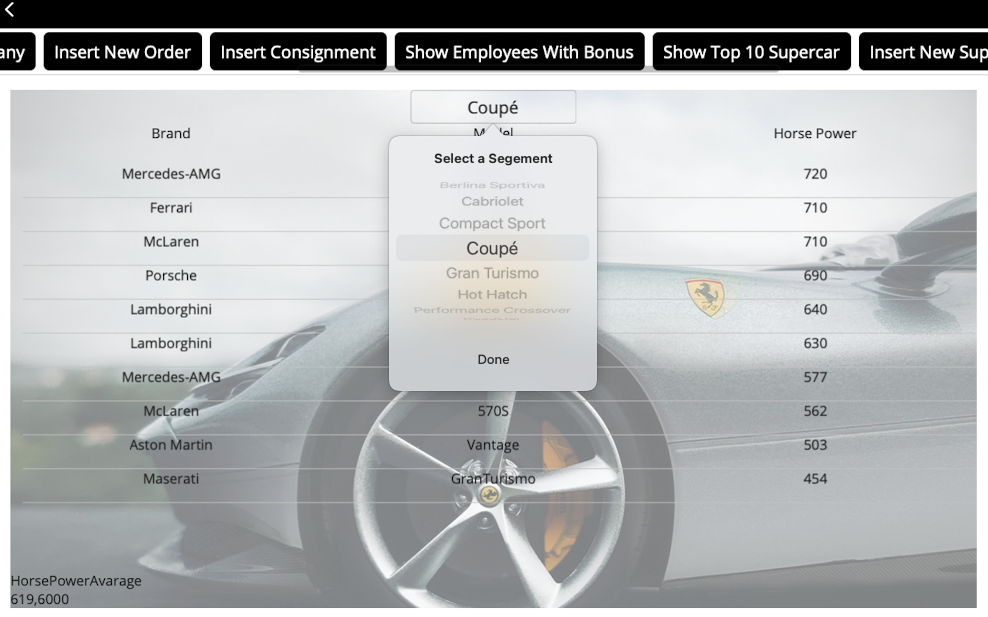
\includegraphics[width=\linewidth]{images/app/topTenSupercar.png}
\end{center}

\subsubsection{Pagina di visualizzazione degli ordini di un cliente}
Questa schermata permette l'inserimento del codice presente nel badge del cliente, 
in seguito si andranno inserite la data di inizo e fine periodo da valutare.

Si presenterà quindio una tabella con le vetture acquistate dal cliente in quel periodo.

\begin{center}
    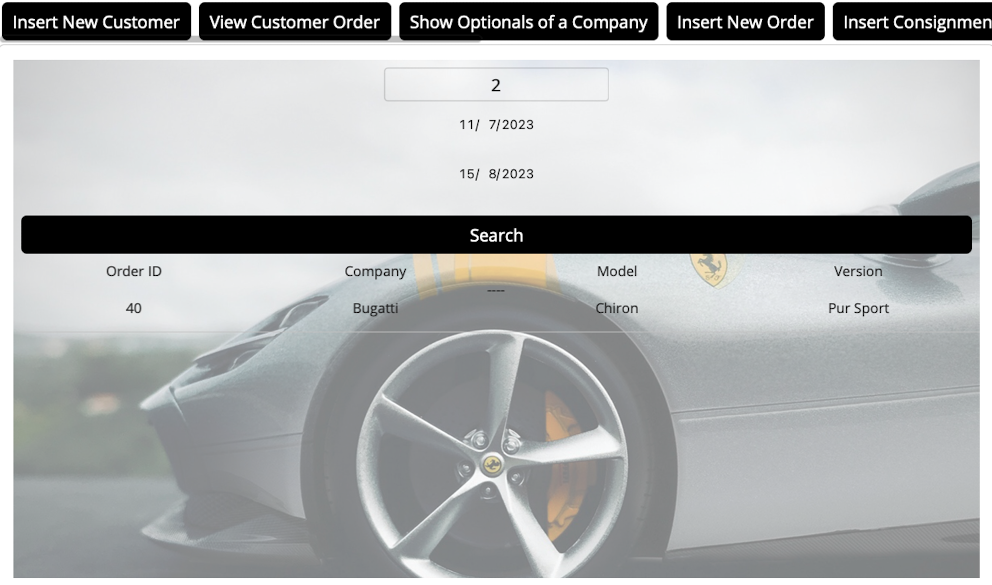
\includegraphics[width=\linewidth]{images/app/showOrders.png}
\end{center}

\subsubsection{Pagina di visualizzazione degli optional di un produttore}
Con l'utilizzo del menu a tendina si può scegliere un produttore e in seguito
visualizzare gli optional di cui la concessionaria ha disponibilità.

\begin{center}
    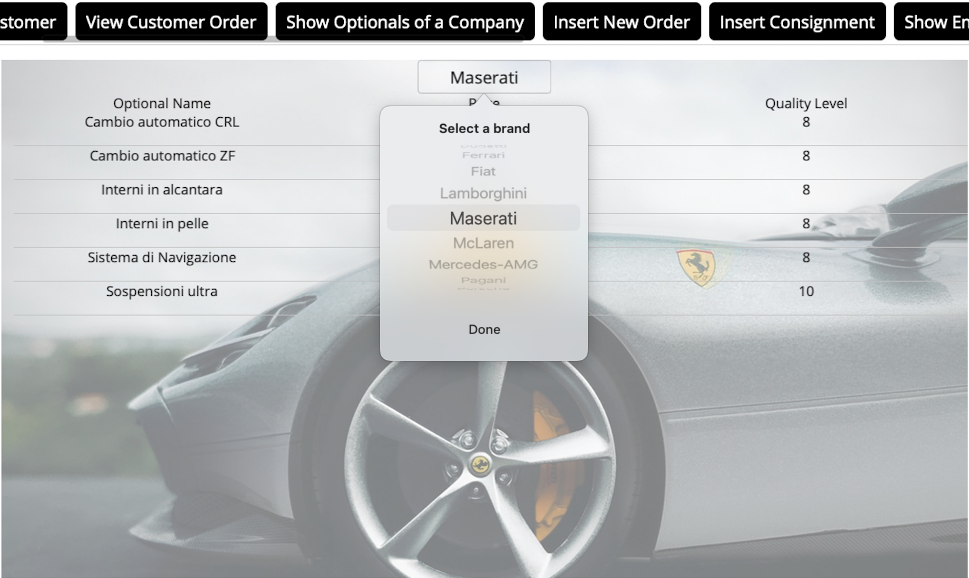
\includegraphics[width=\linewidth]{images/app/brandOptional.png}
\end{center}

\subsubsection{Pagina di visualizzazione della spesa annuale}
Inserendo un anno avremo il calcolo della spesa annuale in risorse umane della
concessionaria.
Vengono tenuti in considerazione sia gli stipendi che i bonus.

\begin{center}
    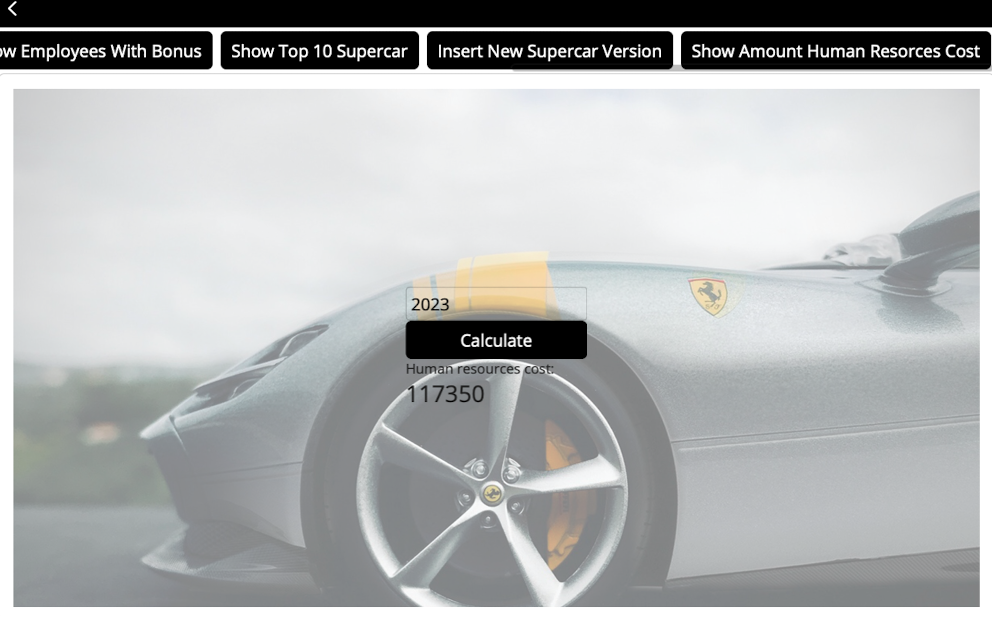
\includegraphics[width=\linewidth]{images/app/humanResourcesCost.png}
\end{center}

\subsubsection{Pagina di inserimento di un nuovo cliente}
Questa schermata permette l'inserimento di un nuovo cliente.

Il pulsante 'Insert' è capace di segnalare se la query è andata a buon fine o meno.

\begin{center}
    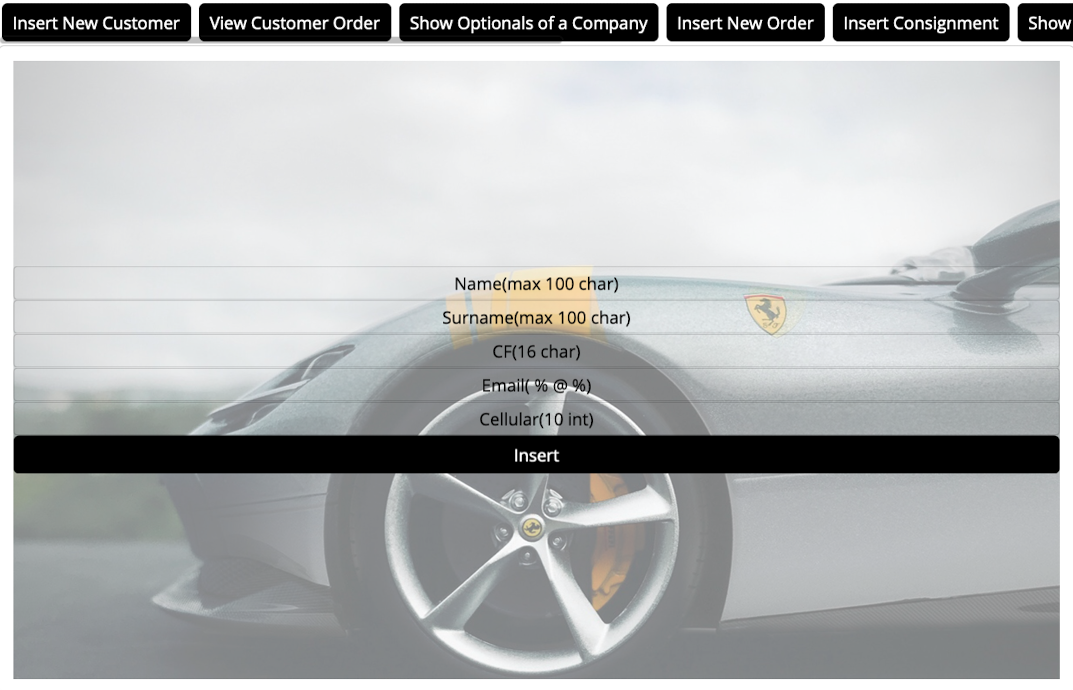
\includegraphics[width=\linewidth]{images/app/insertCostumer.png}
\end{center}

\subsubsection{Pagina di inserimento di un nuovo ordine}
Di seguito troviamo la pagina di creazione di un ordine e calcolo della spesa
totale. I menu a tendina vengono aggiornati in tempo reale basandosi sul valore
scelto nel menu precedente.

E' possibile inserire più vetture nello stesso ordine e per ogni vettura si
possono inserire più optional che vengono filtrati per il segmento al quale
appartiene la vettura.

Da notorsi che alla scelta di una vettura o optional vengono aggiornati anche i
menu a tendina successivi non presentando più le voci già scelte.

\begin{center}
    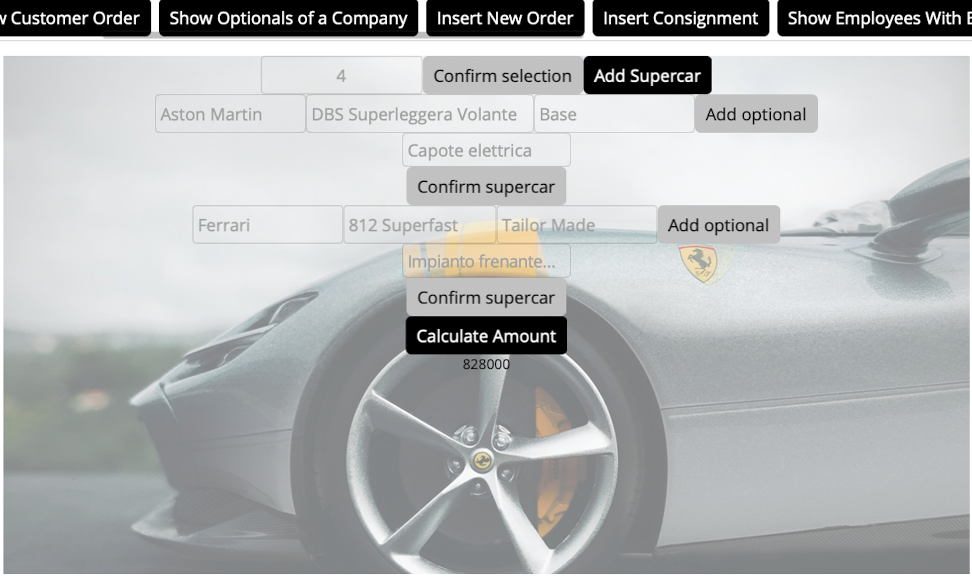
\includegraphics[width=\linewidth]{images/app/addOrder.png}
\end{center}

\subsubsection{Pagina di visualizzazione dei migliori dipendenti}
Nella seguente schermata è possibile scegliere un mese ed un anno per poi
visualizzareuna tabella con i dipendenti che hanno ottenuto il bonus in quel
periodo.

\begin{center}
    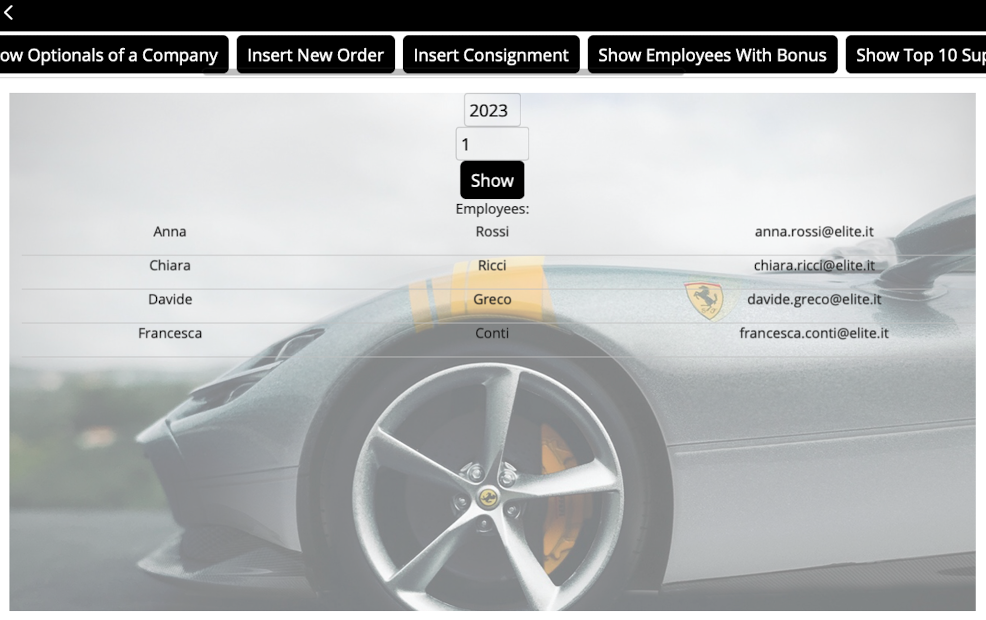
\includegraphics[width=\linewidth]{images/app/bestEmployees.png}
\end{center}

\end{document}

